\documentclass{beamer}
\usetheme{Warsaw}
\graphicspath{{figuras/}}
\setbeamercolor{normal text}{fg=white,bg=black!90}
\setbeamercolor{structure}{fg=white}

\setbeamercolor{alerted text}{fg=red!85!black}

\setbeamercolor{item projected}{use=item,fg=black,bg=item.fg!35}

\setbeamercolor*{palette primary}{use=structure,fg=structure.fg}
\setbeamercolor*{palette secondary}{use=structure,fg=structure.fg!95!black}
\setbeamercolor*{palette tertiary}{use=structure,fg=structure.fg!90!black}
\setbeamercolor*{palette quaternary}{use=structure,fg=structure.fg!95!black,bg=black!80}

\setbeamercolor*{framesubtitle}{fg=white}

\setbeamercolor*{block title}{parent=structure,bg=black!60}
\setbeamercolor*{block body}{fg=black,bg=black!10}
\setbeamercolor*{block title alerted}{parent=alerted text,bg=black!15}
\setbeamercolor*{block title example}{parent=example text,bg=black!15}
\setbeamercolor{figure text}{fg=black}

\setbeamertemplate{headline}{}

\usepackage[brazil,spanish]{babel}
\usepackage[utf8]{inputenc}
\usepackage{color}
\usepackage{listings}
\usepackage{setspace}
\usepackage{graphicx}

%%%%%%%%%%%%%%%%%%%%%%%%%%%%%%%%%%%%%%%%%%%%%%%%



\title[Defensa de Memoria]{\bf An\'alisis de Im\'agenes a trav\'es de la Transformaci\'on de Box-Cox}
% Titre du diaporama

% Sous-titre optionnel

\author{Fabián Castellano Núñez}
% La commande \inst{...} Permet d'afficher l' affiliation de l'intervenant.
% Si il y a plusieurs intervenants: Marcel Dupont\inst{1}, Roger Durand\inst{2}
% Il suffit alors d'ajouter un autre institut sur le modèle ci-dessous.

\institute[Universidad Técnica Federico Santa María]
  {
  Profesor Guia: Ronny Vallejos A.
  }


\date{Marzo,  2024}
% Optionnel. La date, généralement celle du jour de la conférence

\subject{Transformación Box-Cox}
% C'est utilisé dans les métadonnes du PDF
\titlegraphic{
    
\includegraphics[width=3cm,keepaspectratio]{logo_dmat.png}%
    \hfill%
    
\includegraphics[width=2cm,keepaspectratio]{logo_usm3.png}%
}
%%%%%%%%%%%%%%%%%%%%%%%%%%%%%%%%%%%%%%%%%%%%%%%%%%%%%%%%%%%%%%%%%%%%%
\begin{document}

\begin{frame}
  \titlepage
\end{frame}
\begin{frame}
    \begin{center}
        {\LARGE\bf Introducción}
    \end{center}
\end{frame}

\begin{frame}{Introducción}
    % \pause
    \begin{itemize}
        \item Se evalua el uso de la transformación Box-Cox para en im\'agenes. Solo se ha aplicado en este contexto por Lee et al. y Cheddad.
        % \pause
        \item La transformación Box-Cox, se utiliza para asemejar datos a una Distribución Normal.
        % \pause
        \item Se estudia la relación entre las im\'agenes y sus transformadas, utilizabndo métodos de correlación como $dCor$, $MIC$, y $\rho$.
    \end{itemize}

    \begin{figure}
        % \pause
        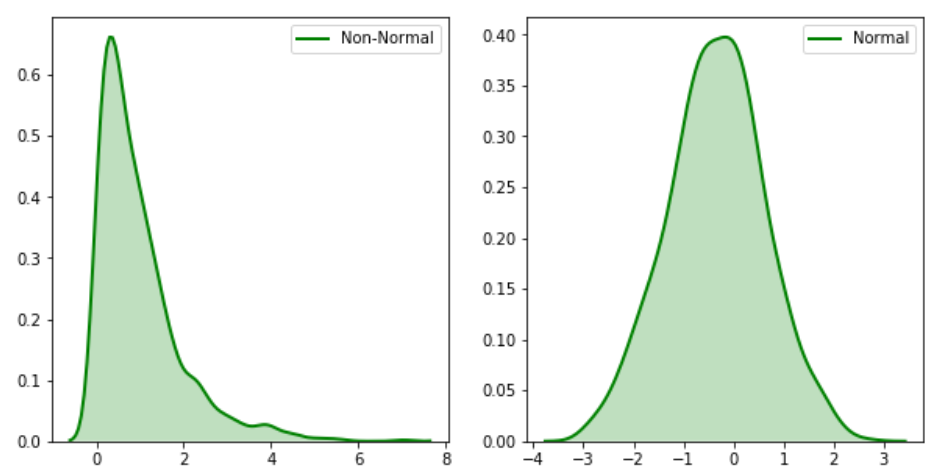
\includegraphics[width=0.5\textwidth]{output275.png}
        \hfill
        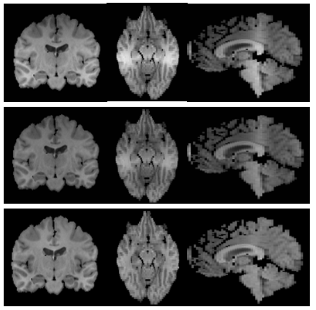
\includegraphics[width=0.4\textwidth]{brains.png}
    \end{figure}
\end{frame}


\begin{frame}{Contenidos}
  \tableofcontents
  % possibilité d'ajouter l'option [pausesections]
\end{frame}

\begin{frame}
    \begin{center}
        {\LARGE\bf Coeficientes de Correlación}
    \end{center}
\end{frame}

\section{Coeficientes de Correlación}
\subsection{Coeficiente de Información Máxima}
\begin{frame}{Coeficiente de Información Máxima}
    % \pause
    \begin{itemize}
        \item El coeficiente de información máxima (MIC) es un coeficiente de correlación no paramétrico que mide la relación entre dos variables aleatorias.
        \item Propuesto por Reshef en 2011 en "Detecting Novel Associations in Large Data Sets"
        \item Se basa en la idea de que una relación fuerte entre dos variables debería ser capaz de predecir una a partir de la otra de manera precisa.
        \item Permite detectar relaciones débiles pero importantes.
    \end{itemize}
    % \pause
    \begin{block}{Información mutua}
    Dada una distribución bivariada $P(x,y)$, definimos:
        \begin{equation}
            \mathrm{I}(X ; Y)=\int_{\mathcal{Y}} \int_{\mathcal{X}} P_{(X, Y)}(x, y) \log \left(\frac{P_{(X, Y)}(x, y)}{P_{X}(x) P_{Y}(y)}\right)dxdy
        \end{equation}
    \end{block}
\end{frame}

\begin{frame}{Coeficiente de Información Máxima}
    Sea D un conjunto finito de pares ordenados, podemos particionar los valores de la primera coordenada en x contenedores, y los valores de la segunda en y de estos y generar una mmalla $G$ de $x \times y$ celdas.
    \begin{block}{Distribución inducida por una malla}
        Dado una malla $G$, llamaremos $D|_G$ la distribuci\'on inducida por los puntos de $D$ en las celdas de $G$, i.e., la distribuci\'on en las celdas de $G$ obtenida al dejar que la funci\'on de densidad de probabilidad en cada celda sea la fracci\'on de puntos de $D$ que caen en esa celda.
    \end{block}
    \begin{figure}[H]
        \centering
        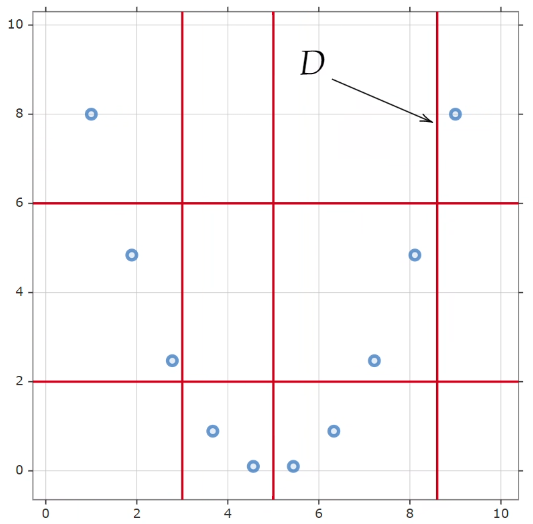
\includegraphics[width=0.3\textwidth]{mallaG4x3.png}
    \end{figure}
\end{frame}

\begin{frame}{Coeficiente de Información Máxima}
    % \pause
    \begin{figure}[H]
        \centering
        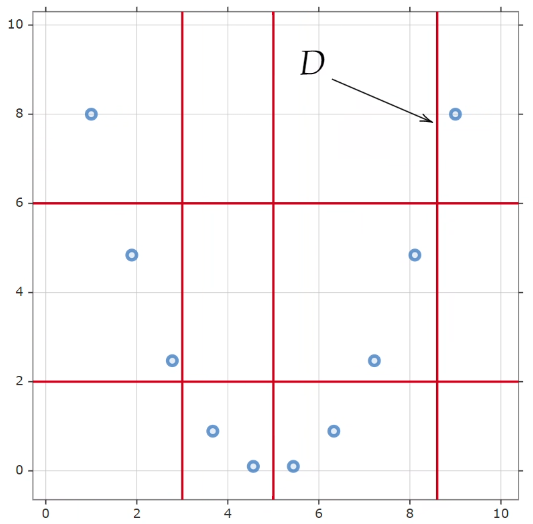
\includegraphics[width=0.3\textwidth]{mallaG4x3.png}
    \end{figure}
    % \pause
    \begin{block}{Densidad}
        Para la malla definica en la figura, definimos la función de densidad como:
        \begin{equation}
            f_{D|_G}(i,j) = \left\{\begin{array}{lr}
                \frac{1}{10} & \text{si } (i,j) \in \{ (1,3), (4,1)\} \\
                \frac{2}{10}, & \text{si }(i,j) \in \{ (1,2), (2,1), (3,1),(3,2)\}  \\
                0, & \text{Otro caso.}
                \end{array}\right.
        \end{equation}
    \end{block}
\end{frame}


\begin{frame}{Coeficiente de Información Máxima}
    % \pause
    \begin{block}{Máximo sobre todas las mallas}
        Para un conjunto finito $D\in\mathcal{R}  ^2$ y enteros positivos $x,y$, definimos:
        $$
        I^*(D,x,y)=\max I(D|_G)
        $$
    \end{block}
    % \pause
    \begin{block}{Matriz Característica}
        Definimos la siguiente matriz       
        \begin{equation}
	    	M(D)_{x, y}=\frac{I^{*}(D, x, y)}{\log \min \{x, y\}}
        \end{equation}
        Notemos que en principio la matriz es infinita.
    \end{block}
\end{frame}


\begin{frame}{Coeficiente de Información Máxima}
     
    % \pause
    \begin{block}{Coeficiente de Información Máxima}
        Definido en por Reshef en 2011 Dado un conjunto de datos bivariado, tenemos:
        \begin{equation}
	    	\operatorname{MIC}(D)=\max _{x y<B(n)}\left\{M(D)_{x, y}\right\}
        \end{equation}
        donde $\omega(1)<B(n) \leq O\left(n^{1-\varepsilon}\right)$ para alg\'un $0<\varepsilon<1$. En el artiuclo utilizan $B(n)=n^{0.6}$
    \end{block}
\end{frame}


\begin{frame}{Coeficiente de Información Máxima}
    % \pause
    ¿Cómo calculamos el MIC en la práctica?
    % \pause
    \begin{figure}
        \centering
        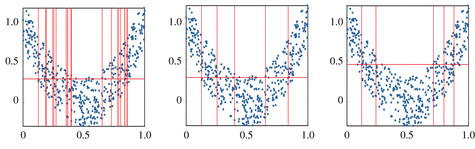
\includegraphics[width=0.4\textwidth]{rsos201424f03.png}
    \end{figure}
\end{frame}


\subsection{Correlaci\'on y Covarianza por Distancia}

\begin{frame}{Correlaci\'on por Distancia}
    % \pause
    Esta se Plantea como una generalizaci\'on de la correlaci\'on de Pearon, en particular cumple:
    \begin{enumerate}
        \item $\mathcal{R}(X,Y)$ est\'a definido para $X,Y$ de dimensi\'on aleatoria.
        \item $\mathcal{R}(X,Y) = 0$ caracteriza la independenc\'a de $X$ e $Y$.
        \item Busca encontrar relaciones no lineales entre dos conjuntos de datos, en particular establecer una forma de caracterizar independencía
        entre dos distribuciónes.
    \end{enumerate}
    % \pause
    \begin{block}{Correlaci\'on por Distancia}
        La Covarianza por distancia (dCov) entre los vectores aleatorios $X$ e $Y$ con primeros momentos finitos es el n\'umero no negativo $\mathcal{V}(X, Y)$ definido por:
        \begin{equation}
            \begin{aligned}\label{dcov_formula}
                \mathcal{V}^2(X, Y) & =\left\|f_{X, Y}(t, s)-f_X(t) f_Y(s)\right\|^2 \\
                & =\frac{1}{c_p c_q} \int_{\mathcal{R}^{p+q}} \frac{\left|f_{X, Y}(t, s)-f_X(t) f_Y(s)\right|^2}{|t|_p^{1+p}|s|_q^{1+q}} d t d s .
                \end{aligned}
        \end{equation}
    \end{block}
\end{frame}


\begin{frame}{Correlaci\'on por Distancia}
    % \pause
    \begin{block}{Varianza por distancia}
        Se define como la raiz cuadrada:

        $$
        \mathcal{V}^2(X)=\mathcal{V}^2(X, X)=\left\|f_{X, X}(t, s)-f_X(t) f_X(s)\right\|^2 .
        $$
    
        Por definici\'on de la norma $\|\cdot\|$, es claro que  $\mathcal{V}(X, Y) \geq 0$ y $\mathcal{V}(X, Y)=0$ si y solo si $X$ e $Y$ son indepentes.
        
    \end{block}
    % \pause
    \begin{block}{Correlaci\'on por Distancia}
        La correlaci\'on por distancia (dCor) entre los vectores aleatorios $X$ e $Y$ con primer momento finito es el n\'unero no negtivo $\mathcal{R}(X, Y)$ definido por:
		$$
		\mathcal{R}^2(X, Y)= \begin{cases}\frac{\mathcal{V}^2(X, Y)}{\sqrt{\mathcal{V}^2(X) \mathcal{V}^2(Y)}}, & \mathcal{V}^2(X) \mathcal{V}^2(Y)>0 \\ 0, & \mathcal{V}^2(X) \mathcal{V}^2(Y)=0\end{cases}.
		$$
    \end{block}
\end{frame}

\begin{frame}{Correlaci\'on por Distancia}
    Ahora, para el caso muestral, definimos $\left(a_{k l}\right)=\left(\left|X_k-X_l\right|_p\right)$ y $\left(b_{k l}\right)=\left(\left|Y_k-Y_l\right|_q\right)$. Definimos:

	$$
	A_{k l}=a_{k l}-\bar{a}_{k .}-\bar{a}_{. l}+\bar{a}_{. .}, \quad k, l=1, \ldots, n,
	$$
	donde
	$$
	\bar{a}_{k .}=\frac{1}{n} \sum_{l=1}^n a_{k l}, \quad \bar{a}_{. l},=\frac{1}{n} \sum_{k=1}^n a_{k l}, \quad \bar{a}_{. .}=\frac{1}{n^2} \sum_{k, l=1}^n a_{k l} .
	$$
	
	De forma analoga, definimos $B_{k l}=b_{k l}-\bar{b}_{k .}-\bar{b}_{\cdot l}+\bar{b}_{. .}$, para $k, l=1, \ldots, n$.
\end{frame}

\begin{frame}{Correlaci\'on por Distancia}
        \begin{block}{Correlaci\'on por Distancia muestral}
            La no negativa Covarianza por distancia muestral $\mathcal{V}_n(\mathbf{X}, \mathbf{Y})$ y la Correlaci\'on por distancia muestral $\mathcal{R}_n(\mathbf{X}, \mathbf{Y})$ estan definidas por
            $$
            \mathcal{V}_n^2(\mathbf{X}, \mathbf{Y})=\frac{1}{n^2} \sum_{k, l=1}^n A_{k l} B_{k l},
            $$
            y
            $$
            \mathcal{R}_n^2(\mathbf{X}, \mathbf{Y})= \begin{cases}\frac{\mathcal{V}_n^2(\mathbf{X}, \mathbf{Y})}{\sqrt{\mathcal{V}_n^2(\mathbf{X}) \mathcal{V}_n^2(\mathbf{Y})}}, & \mathcal{V}_n^2(\mathbf{X}) \mathcal{V}_n^2(\mathbf{Y})>0 \\ 0, & \mathcal{V}_n^2(\mathbf{X}) \mathcal{V}_n^2(\mathbf{Y})=0\end{cases},
            $$
            respectivamente. Adem\'as la Varianza por distancia muestral $\mathcal{V}_n(\mathbf{X})$ est\'a definida por
            $$
            \mathcal{V}_n^2(\mathbf{X})=\mathcal{V}_n^2(\mathbf{X}, \mathbf{X})=\frac{1}{n^2} \sum_{k, l=1}^n A_{k l}^2 .
            $$
        \end{block}
\end{frame}

\begin{frame}{Coeficientes de Correlación}
    \begin{block}{MIC}
        El coeficiente de información máxima (MIC) es un coeficiente de correlación basado en la idea de que una relación fuerte entre dos variables debería ser capaz de predecir una a partir de la otra de manera precisa. Permite detectar relaciones débiles pero importantes
    \end{block}

    \begin{block}{dCor}
        La Correlaci	ón por Distancia (dCor) es una generalización de la correlación de Pearson que busca encontrar relaciones no lineales entre dos conjuntos de datos, en particular establecer una forma de caracterizar independencía entre dos distribuciónes.
    \end{block}
\end{frame}



\begin{frame}
    \begin{center}
        {\LARGE\bf Análisis y Procesamiento de Imágenes}
    \end{center}
\end{frame}

\section{Análisis y Procesamiento de Imágenes}
\begin{frame}{Análisis y Procesamiento de Imágenes}
    % \pause
    \begin{block}{Representación de una Imagen}
        Una imagen es una representaci\'on visual de un objeto, y se puede definir como una funci\'on bidimensional $f(x,y)$, como se muestra en la siguiente ecuaci\'on:

        $$
        f(x, y)=\left[\begin{array}{cccc}
        f(0,0) & f(0,1) & \cdots & f(0, N-1) \\
        f(1,0) & f(1,1) & \cdots & f(1, N-1) \\
        \vdots & \vdots & & \vdots \\
        f(M-1,0) & f(M-1,1) & \cdots & f(M-1, N-1)
        \end{array}\right]
        $$
    \end{block}
\end{frame}
% \pause
\begin{frame}{Análisis y Procesamiento de Imágenes}
    \begin{figure}[H]
        \centering
        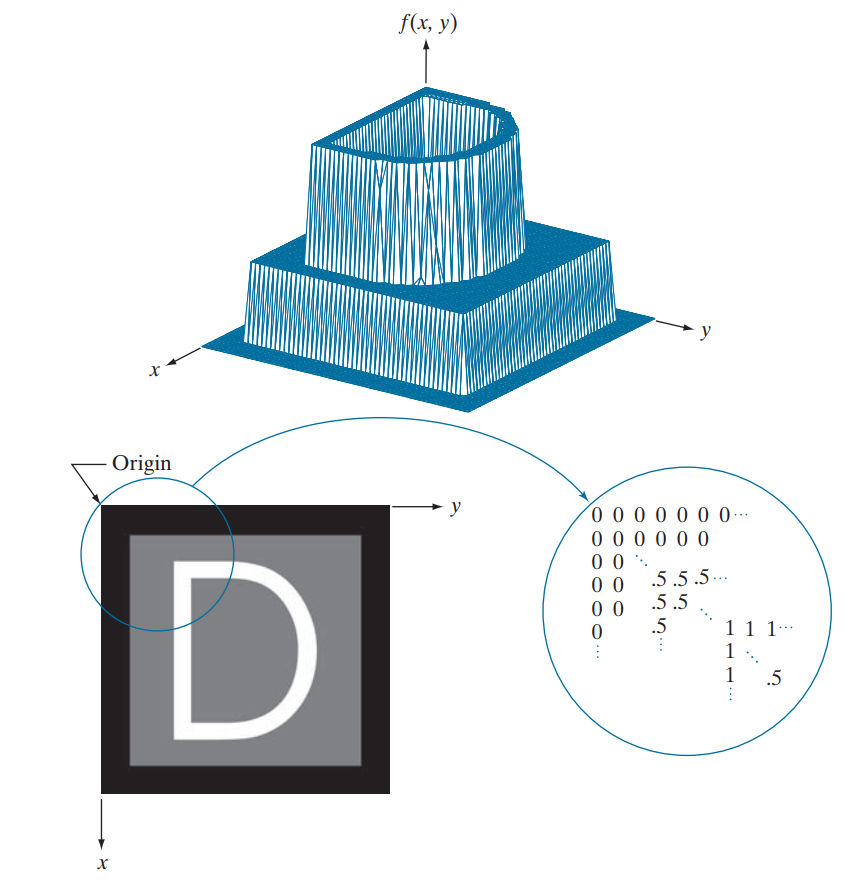
\includegraphics[width=0.4\textwidth]{dip_4_fig2_18.png}
    \end{figure}   
    % \pause     
    (a) Como una superficie.
    (b) Como un conjunto de intensidades visuales.
    (c) Como un conjunto numérico en 2D.
    % \pause
    Notemos que los valores de las intensidades de las imágenes son números enteros entre $[0, 255]$, o numeros reales entre $[0, 1]$.

\end{frame}

\begin{frame}{Banco}
    \begin{figure}[H]
        \centering
        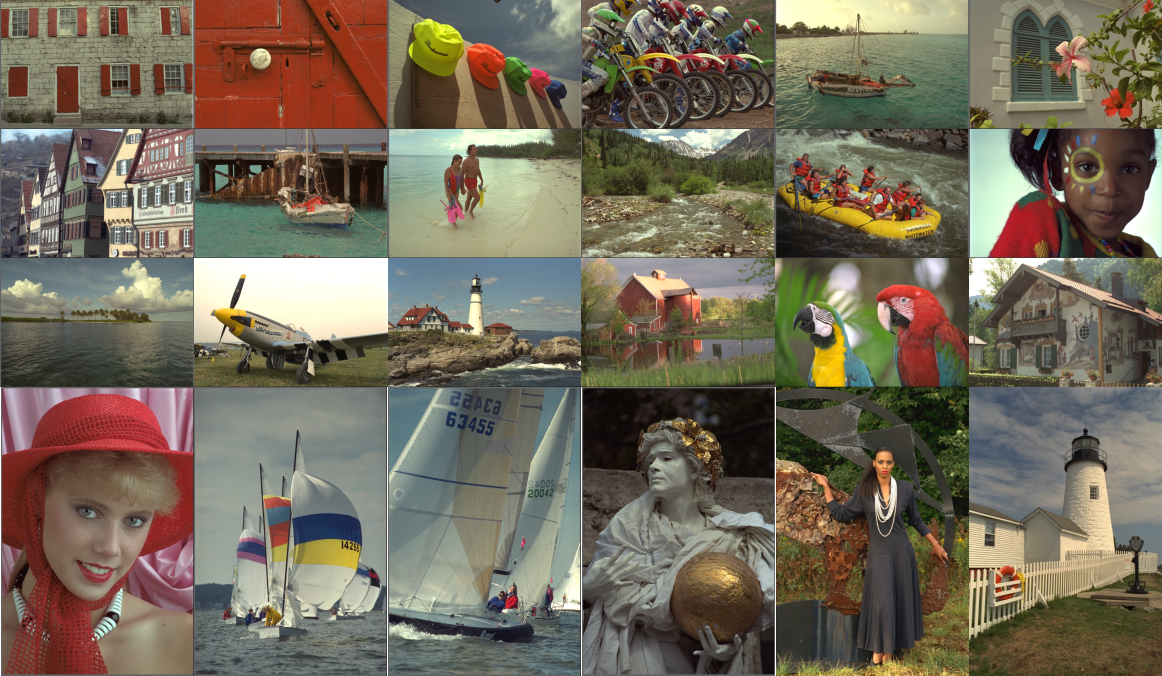
\includegraphics[width=0.8\textwidth]{all_images_grid.png}
        \caption{Banco de im\'agenes a utilizar.}
    \end{figure}        
\end{frame}

\begin{frame}{Análisis y Procesamiento de Imágenes}
    \begin{block}{Im\'agenes Escala de Grises}
        Nos interesa trabajar con escala de grises, lo hacemos de la siguiente forma.

        \begin{equation}
            I(x, y)=0.299 R(x, y)+0.687 G(x, y)+0.114 B(x, y), 
            \label{eq:grayscale}
        \end{equation}

        que corresponde el canal gris del espacio de colores $YC_bC_r$.
    \end{block}
    % \pause
    \begin{figure}[H]
        \centering
        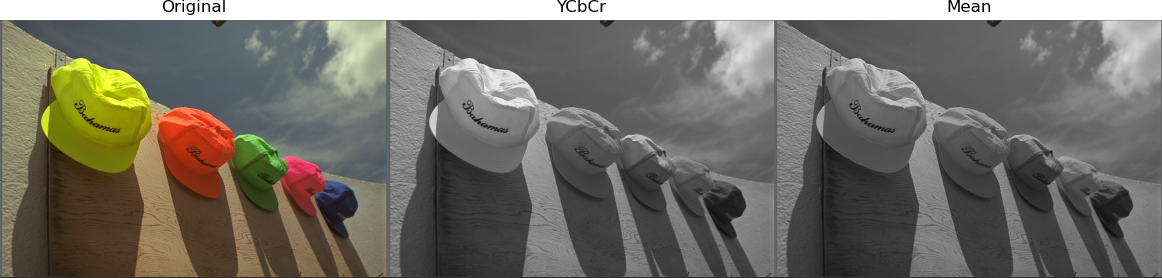
\includegraphics[width=0.8\textwidth]{img_ex_bw.png}
        \caption{Imagen RGB,escala de grises, y promedio simple.}
    \end{figure}
\end{frame}

\begin{frame}{Experimentos Numéricos}
    % \pause
    \begin{figure}[H]
        \centering
        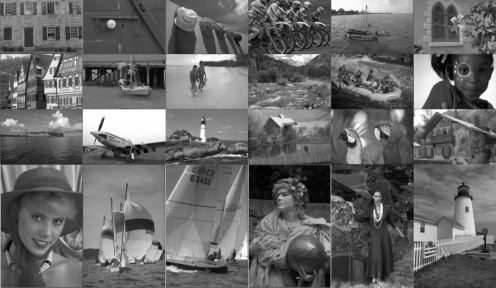
\includegraphics[width=0.8\textwidth]{all_images_grid_bw.png}
        \caption{Banco de im\'agenes a utilizar, en escala de grises.}
    \end{figure}     
\end{frame}

    

\begin{frame}{Correlaci\'on entre Im\'agenes}
    % \pause
    Los métodos de correlación definidos anteriormente están pensados para ser aplicados sobre dos vectores, pero en el caso de imágenes, tenemos una matriz de datos. Por lo tanto, necesitamos una forma de transformar una imagen en un vector unidimensional.
    % \pause
    \begin{block}{Imagen a Vector}
        Dada una imagen $I(x, y)$, la transformamos a un vector unidimensional  $I_{\cdot}(t)$, notemos que para este contexto el ordén no es relevante. Comparamos estos dos vectores.
    \end{block}
    % \pause
    \begin{block}{Histograma}
        Generamos un histograma de los valores de los vectores, con tantos bins como sea necesario. Comparamos estos histogramas.
    \end{block}
\end{frame}

\begin{frame}{Ejemplos}
    % \pause
    \begin{figure}[H]
        \centering
        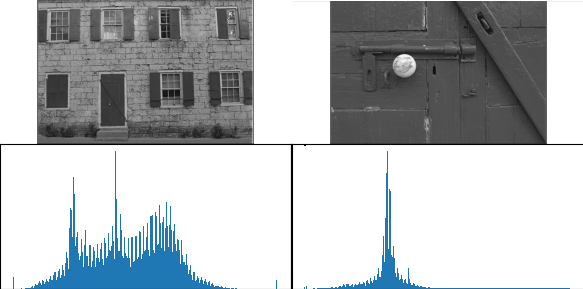
\includegraphics[width=\textwidth]{img_hist.png}
        \caption{Imágenes junto con sus histogramas con ruido.}
    \end{figure}
\end{frame}


\begin{frame}{Correlaci\'on entre Im\'agenes}
    Dado esto, tenemos tenemos 4 formas de comparar dos imágenes:
    \begin{block}{Compración de Imágenes}
        \begin{enumerate}
            \item Comparar los vectores de las imágenes usando MIC.
            \item Comparar los histogramas de las imágenes usando MIC.
            \item Comparar los vectores de las imágenes usando dCor.
            \item Comparar los histogramas de las imágenes usando dCor.
        \end{enumerate}
       
    \end{block}
    Además en los siguientes analisis también se mostrará la correlación de Pearson $\rho$ entre las imágenes, a modo de base de comparación.
\end{frame}
\begin{frame}
    \begin{center}
        {\LARGE\bf Ejemplos}
    \end{center}
\end{frame}

\begin{frame}{Ejemplos}
    % \pause
    \begin{figure}[H]
        \centering
        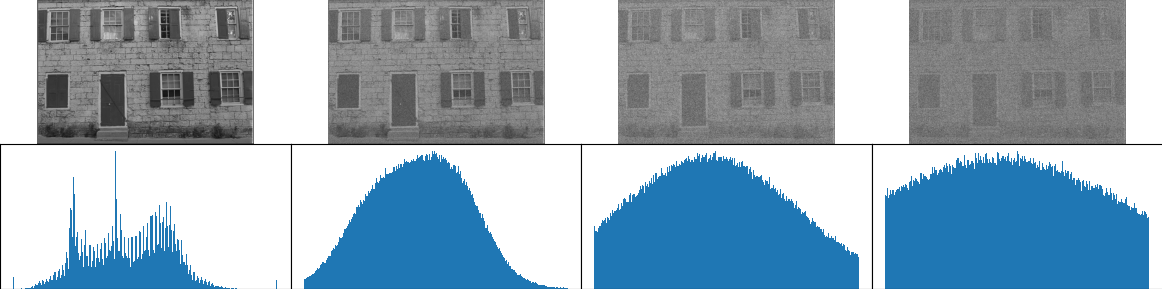
\includegraphics[width=\textwidth]{img_hist_noise_one.png}
        \caption{Imágenes junto con sus histogramas con ruido.}
    \end{figure}
\end{frame}
\begin{frame}{Ejemplos}
    % \pause
    \begin{figure}[H]
        \centering
        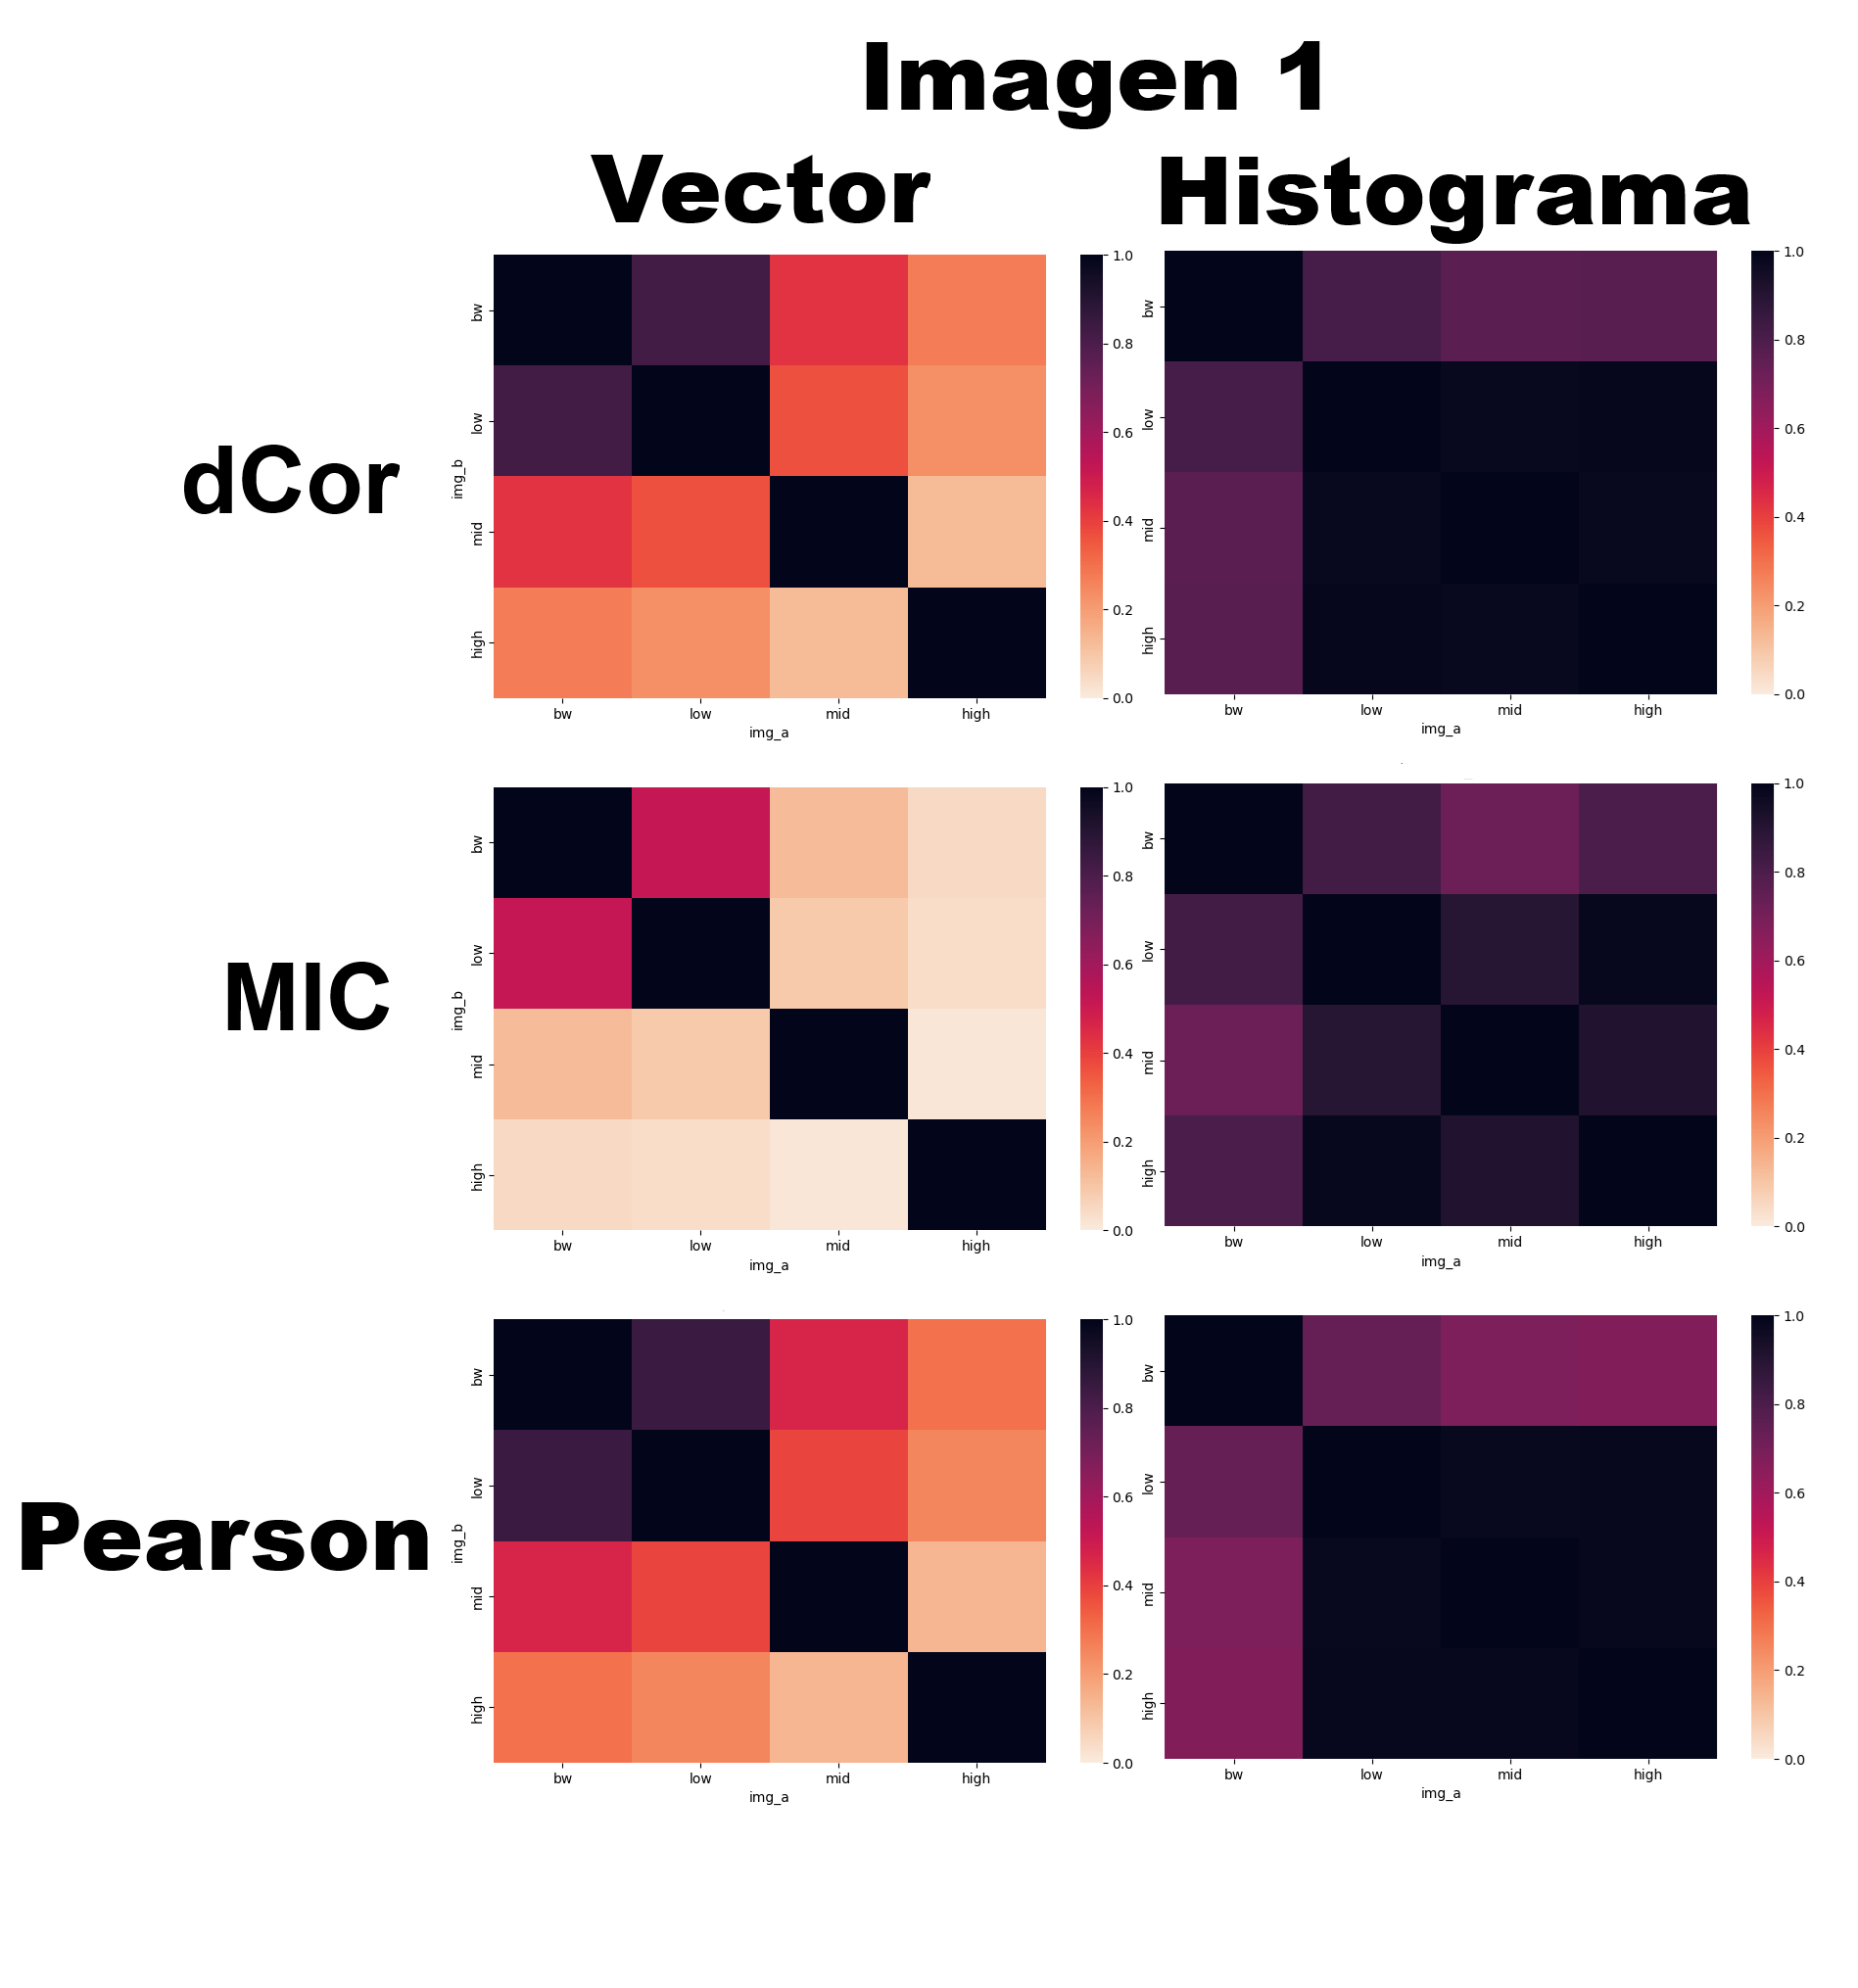
\includegraphics[width=0.4\textwidth]{heatmap_one.png}
        \caption{Matriz de calor para las im\'agenes 1 del banco, cada mapa de calor corresponde a un m\'etodo de comparaci\'on, ya sea comparando el total de la imagen (izquierda), o el histograma de estas (derecha).}
        \label{fig:heatmapall}
    \end{figure}
\end{frame}

\begin{frame}{Ejemplos}
    % \pause
    \begin{figure}[H]
        \centering
        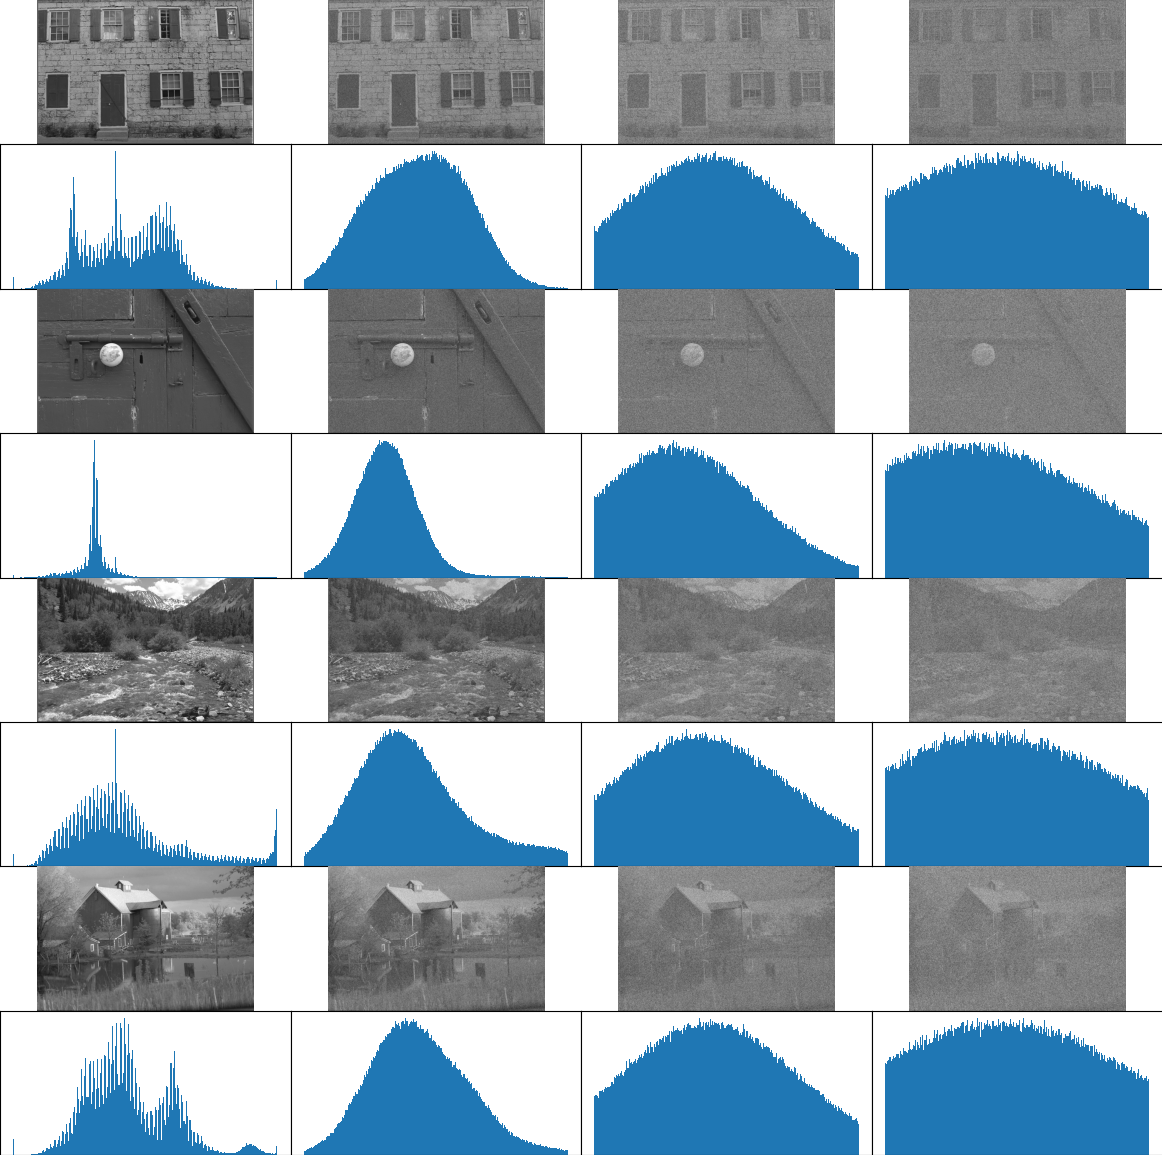
\includegraphics[width=0.6\textwidth]{img_hist_noise.png}
        \caption{Imágenes junto con sus histogramas con ruido.}
    \end{figure}
\end{frame}

\begin{frame}{Ejemplos}
    % \pause
    \begin{figure}[H]
        \centering
        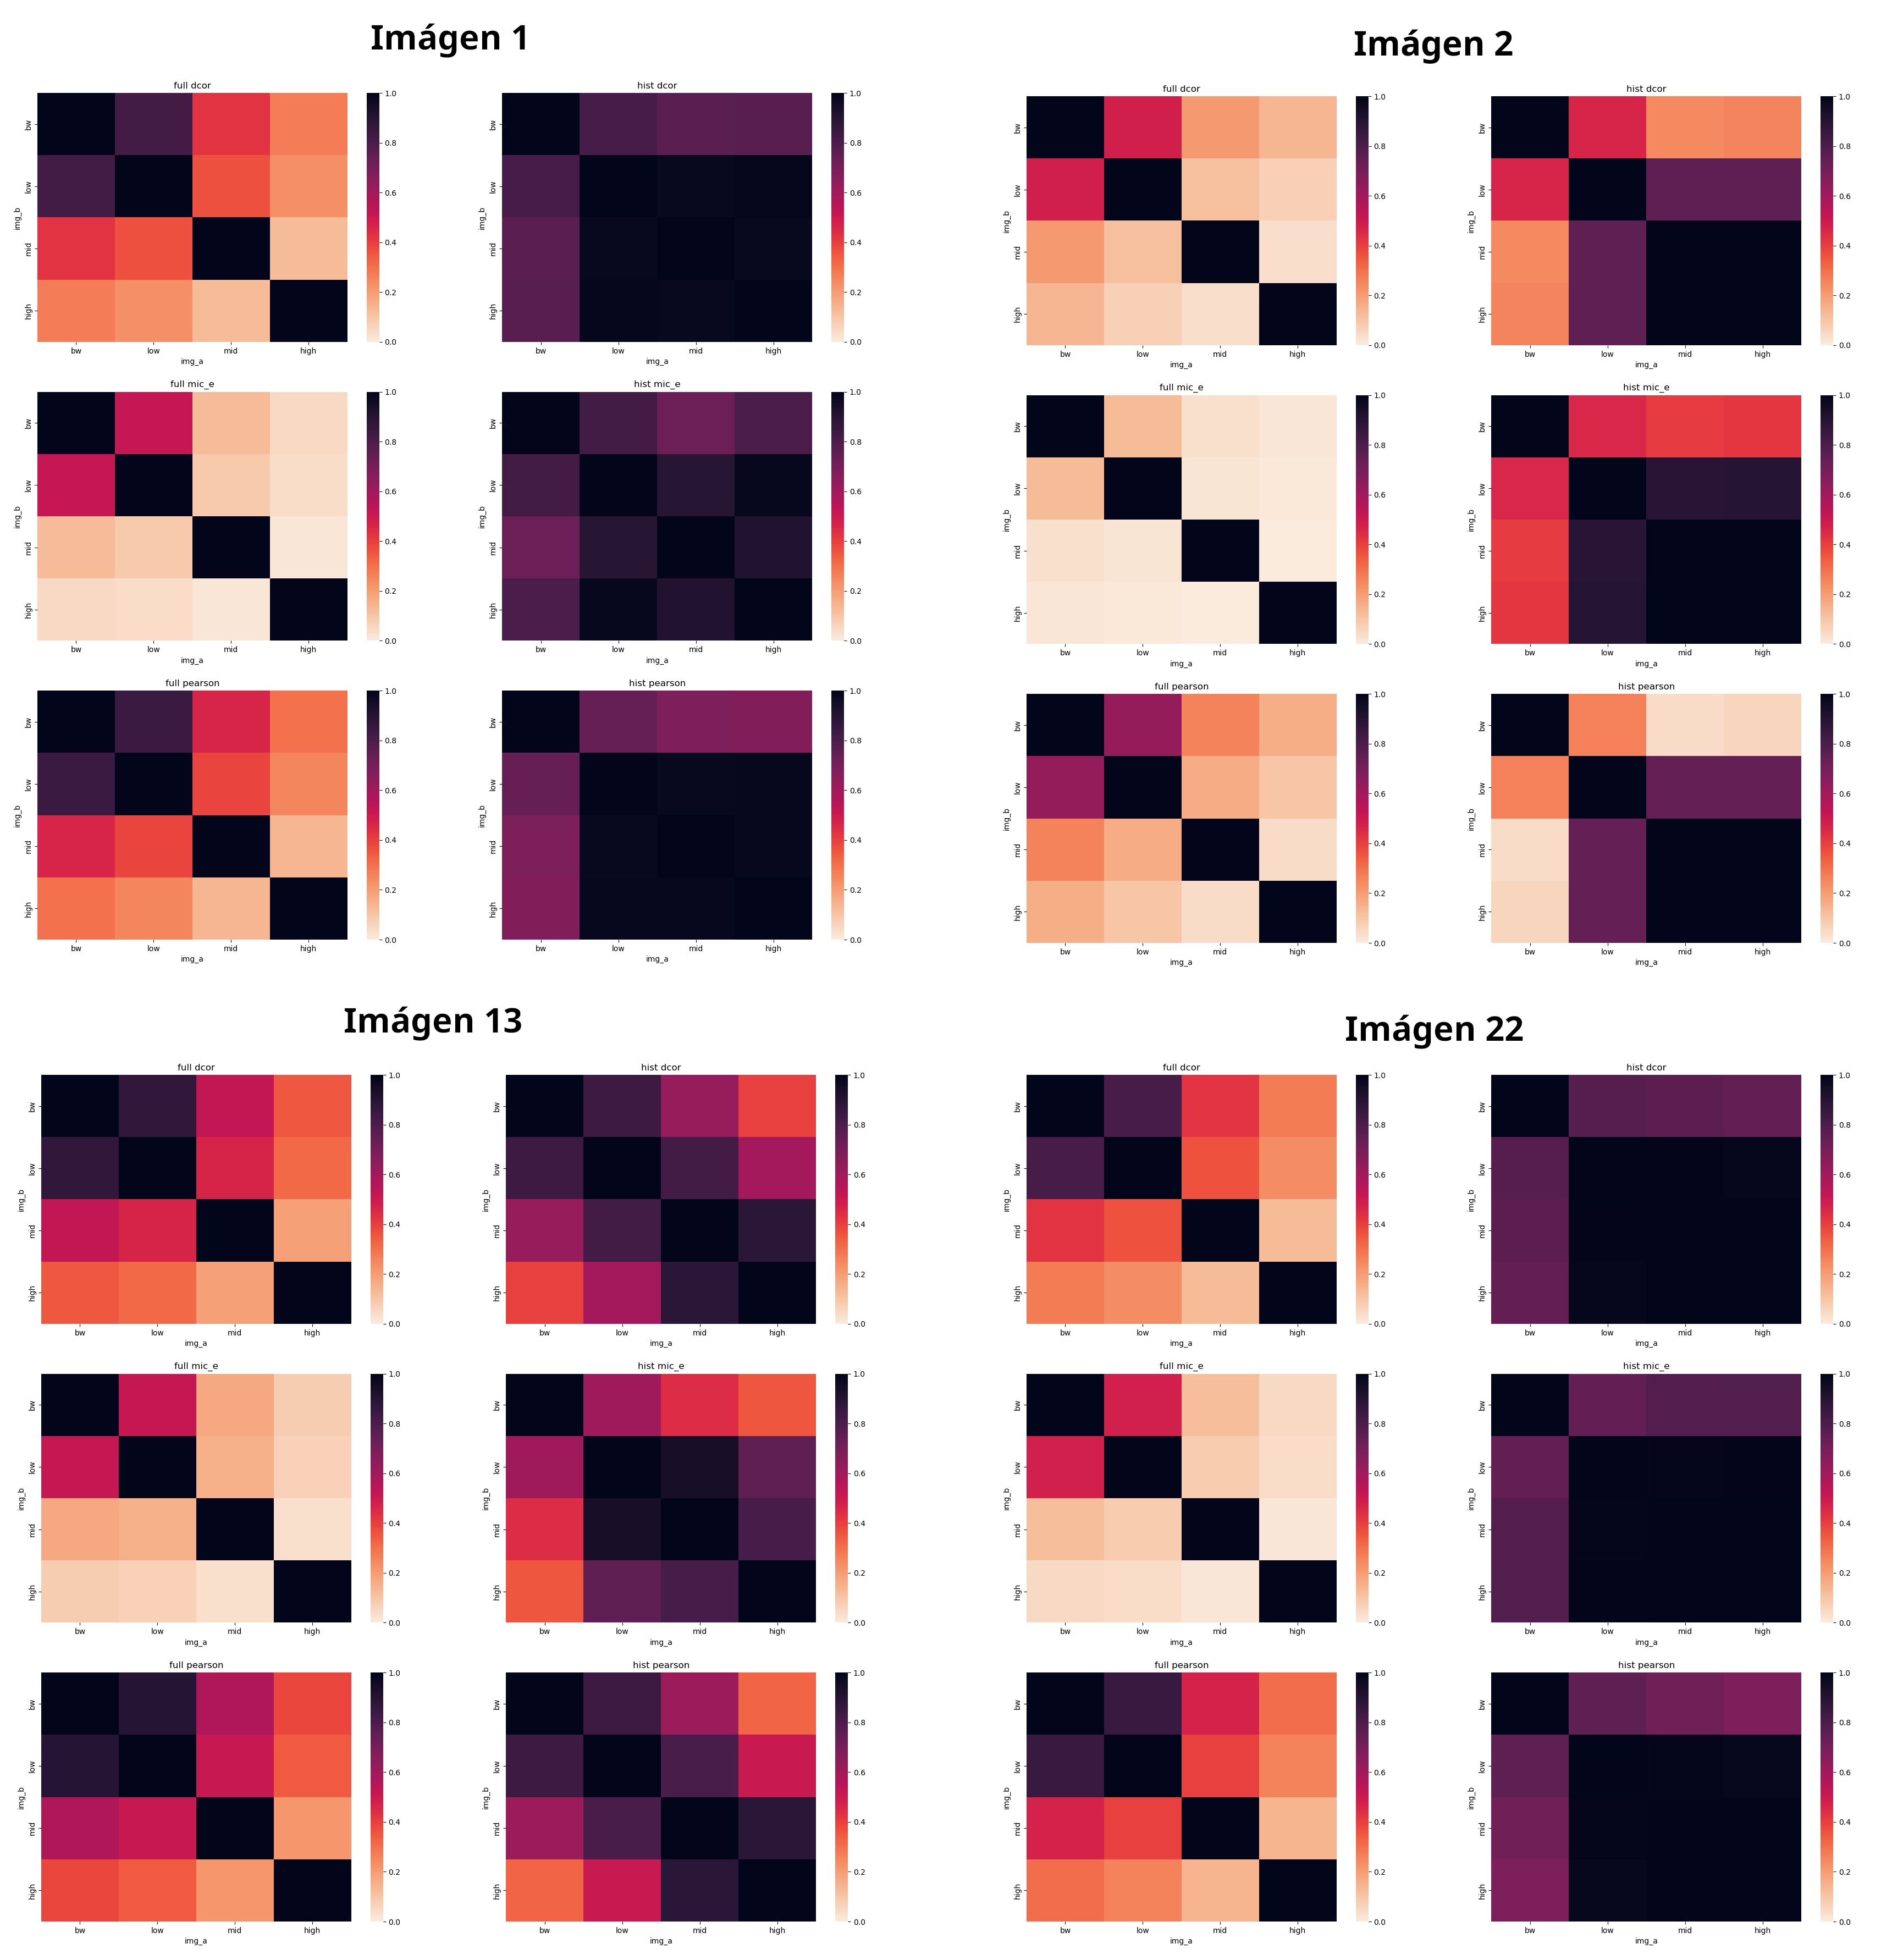
\includegraphics[width=\textwidth]{heatmap_all.png}
        \caption{Matriz de calor para las im\'agenes 1, 2, 13, y 22 del banco, cada mapa de calor corresponde a un m\'etodo de comparaci\'on, ya sea comparando el total de la imagen (izquierda), o el histograma de estas (derecha). La cantidad de ruido aumenta de izquierda a derecha, y de arriba hacía abajo.}
        \label{fig:heatmapall}
    \end{figure}
\end{frame}

\begin{frame}
    \begin{center}
        {\LARGE\bf La transformación Box-Cox}
    \end{center}
\end{frame}

\section{La transformación Box-Cox}

\begin{frame}{La transformación Box-Cox}
    % \pause
    Propuesta por Box y Cox en 1964 en su trabajo "An Analysis of Transformations", la transformación Box-Cox es una familia de transformaciones que se utilizan para hacer que los datos se asemejen a una distribución normal.
    % \pause
    \begin{center}
        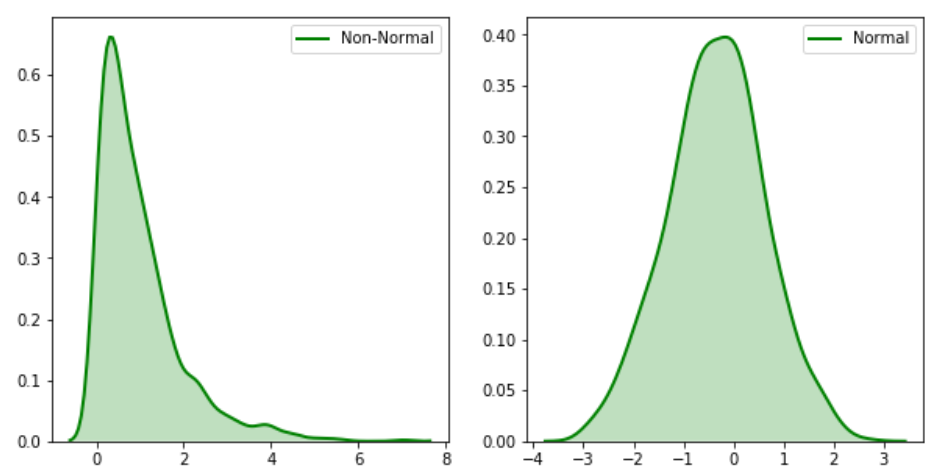
\includegraphics[width=0.5\textwidth]{output275.png}
    \end{center}
    % \pause
    \begin{block}{Transformación Box-Cox}
        Dado un vector $Y=(y_1, y_2, ..., y_n)\in\mathcal{R}_{<0}^n$, la transformación Box-Cox se define como:
        \begin{equation}
            y_i^{(\lambda)}= \begin{cases}\frac{y_i^{\lambda}-1}{\lambda} & (\lambda \neq 0) \\ \log y_i & (\lambda=0)\end{cases}
        \end{equation}
    \end{block}
    % \pause
\end{frame}
\begin{frame}{Transformación Box-Cox}
    ¿Cómo seleccionamos $\lambda$?
    \begin{block}{Verosimilitud}
        \begin{equation*}
            \mathcal{L}(\lambda) \equiv-\frac{n}{2} \log \left[\frac{1}{n} \sum_{j=1}^{n}\left(x_{j}^{\lambda}-\overline{x^{\lambda}}\right)^{2}\right] +(\lambda-1) \sum_{j=1}^{n} \log x_{j}
        \end{equation*}
    \end{block}
    La versimilitud es una función que mide la probabilidad de que los datos observados hayan sido generados por un modelo estadístico. En este caso, la versimilitud mide la probabilidad de que los datos observados hayan sido generados por una distribución normal.

    Notemos que en la práctica, el valor de $\lambda$ se selecciona dentro de un rango de valores como $[-5, 5]$, o $[-2, 2]$.
\end{frame}

\begin{frame}{Box-Cox en Imagenes}
    Tenemos una imagen $I(x, y)$, definimos $\mathcal{F}^{\lambda_{\cdot}}(x, y) = I(x, y)^{(\lambda)}$. Como la transformación Box-Cox aplicada a la intensidad del pixel $(x, y)$.
    % \pause
    \begin{block}{Box-Cox para im\'agenes}
        Sea $\mathcal{F}^{\lambda_{\cdot}}(x, y)$ las im\'agen transformada para alg\'un $\lambda_\cdot$ seleccionado, entonces definimos BCI como:

    \begin{equation}
        BCI = \frac{\left(\mathcal{F}^{\lambda_{\cdot}}(x, y) - \min\left(\mathcal{F}^{\lambda_{\cdot}}(x, y)\right)\right)}{\left(\max\left(\mathcal{F}^{\lambda_{\cdot}}(x, y)\right) - \min\left(\mathcal{F}^{\lambda_{\cdot}}(x, y)\right)\right)}
    \end{equation}
    \end{block}
\end{frame}

% \pause
\begin{frame}{Ejemplos}
    % \pause
    \begin{figure}
        \centering
        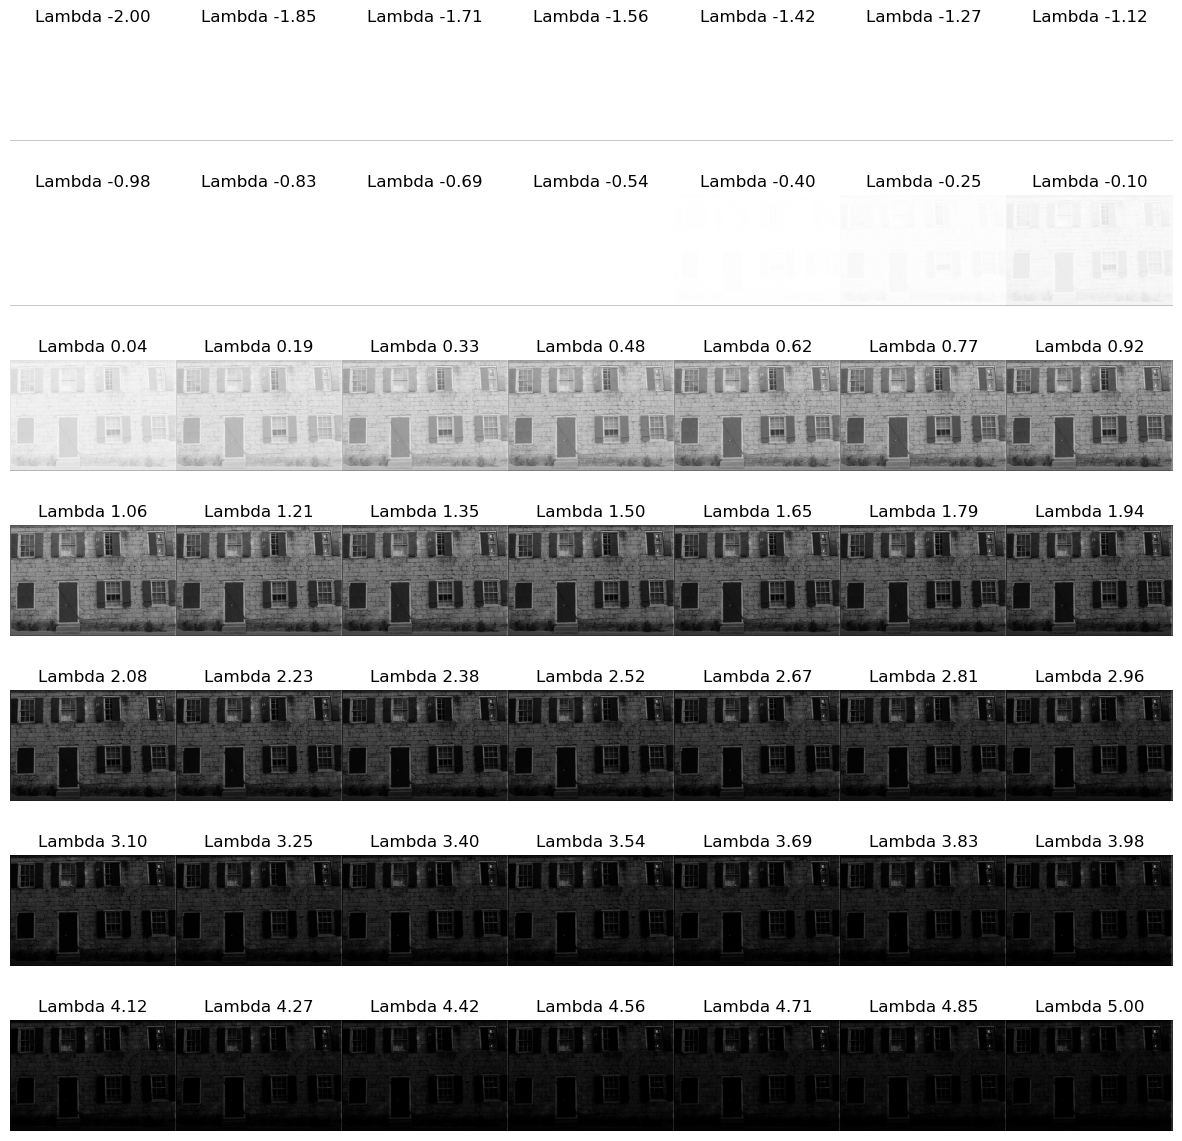
\includegraphics[width=0.6\textwidth]{all_lambda_1.png}
        \caption{Transformaciones de la im\'agen 1.}
        \label{fig:all_lambda_1}
    \end{figure}
\end{frame}


\begin{frame}{Ejemplos}
    % \pause
    \begin{figure}
        \centering
        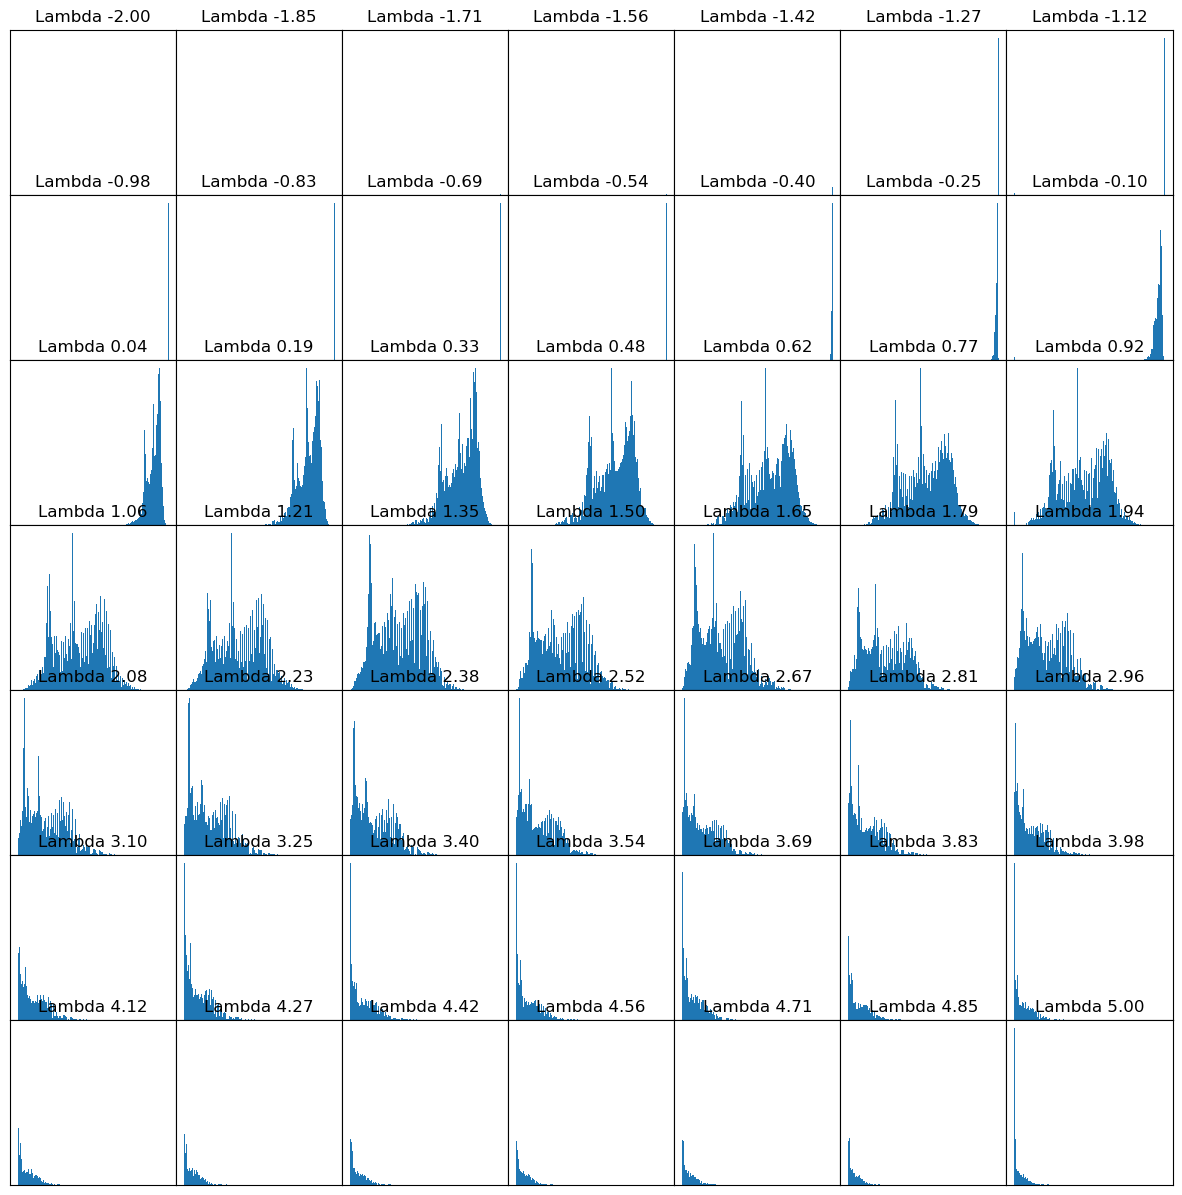
\includegraphics[width=0.6\textwidth]{all_lambda_hist_1.png}
        \caption{Histograma de las transformaciones de la im\'agen 1.}
        \label{fig:img_bci_hist_1}
    \end{figure}
\end{frame}



\begin{frame}{Ejemplos}
    % \pause
    \begin{figure}
        \centering
        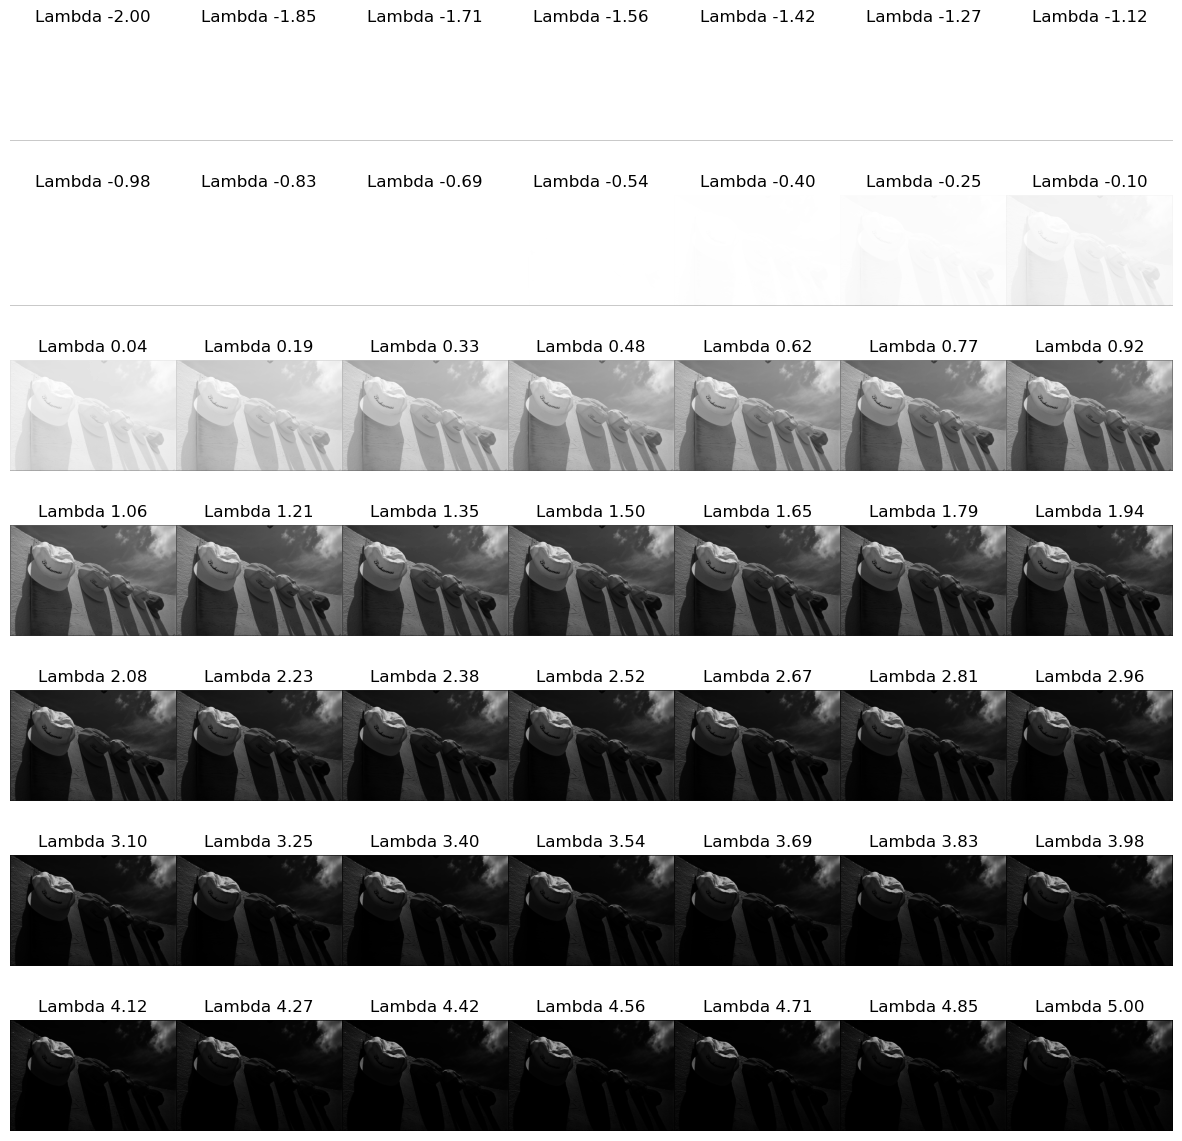
\includegraphics[width=0.6\textwidth]{all_lambda_3.png}
        \caption{Transformaciones de la im\'agen 3.}
        \label{fig:all_lambda_2}
    \end{figure}
\end{frame}

\begin{frame}{Ejemplos}
    % \pause
    \begin{figure}
        \centering
        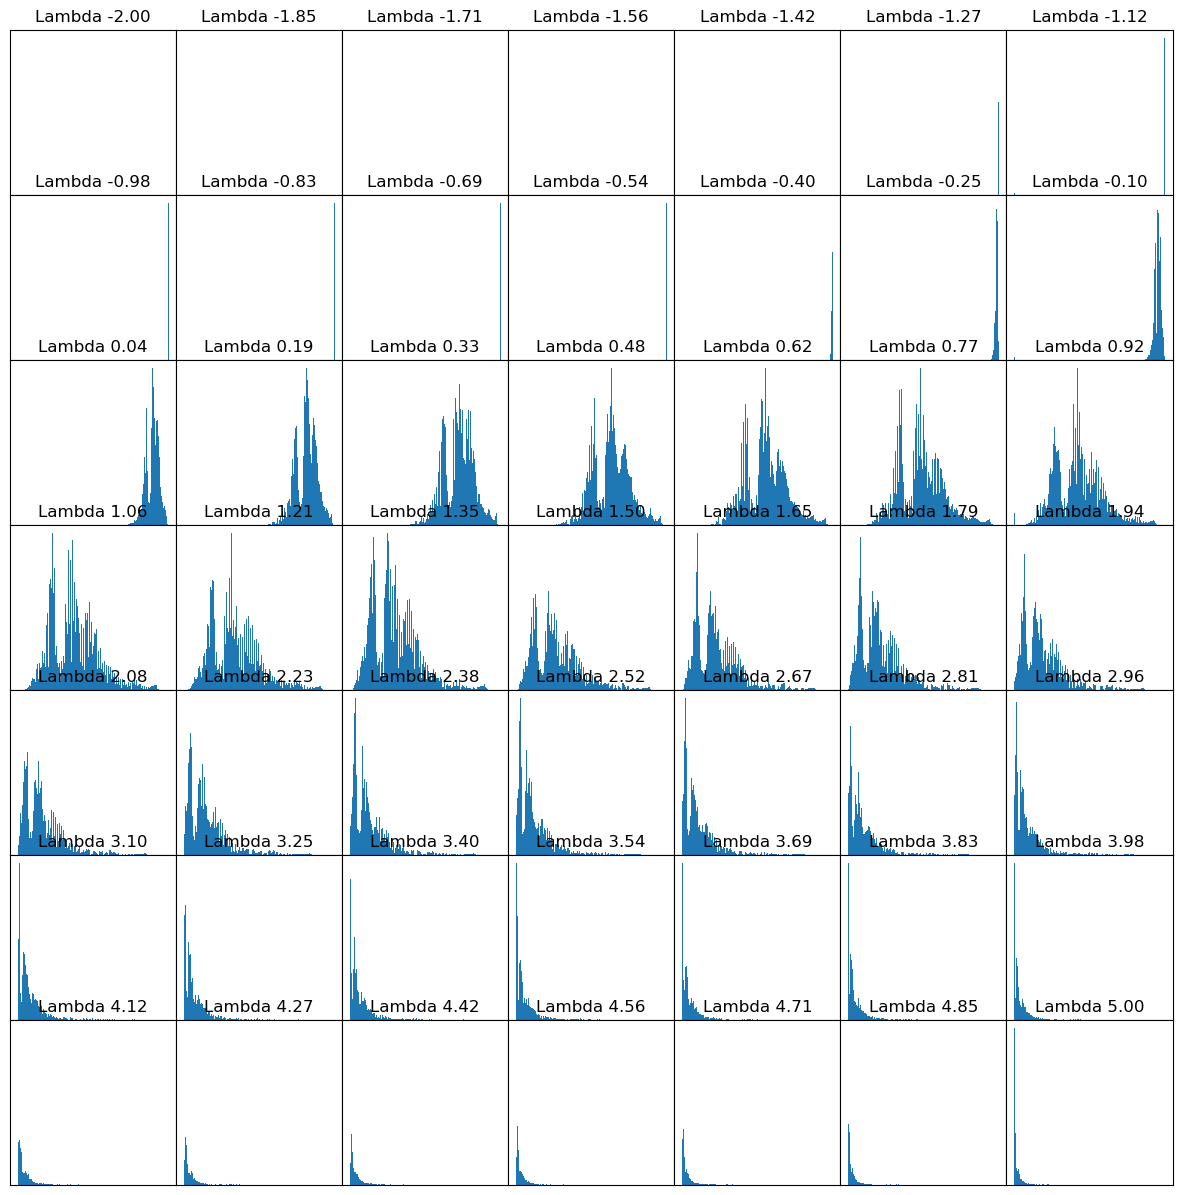
\includegraphics[width=0.6\textwidth]{all_lambda_hist_3.png}
        \caption{Histograma de las transformaciones de la im\'agen 2.}
        \label{fig:img_bci_hist_2}
    \end{figure}
\end{frame}

\begin{frame}
    \begin{center}
        {\LARGE\bf ¿Cómo seleccionamos $\lambda$ para imágenes?}
    \end{center}
\end{frame}

\begin{frame}{Seleccionando $\lambda$ en Im\'agenes}
    % \pause
    \begin{block}{Transformación 1-D}
        Transformar la imagen a un vector unidimensional, usar estos datos para determinar $\lambda$. Propuesto por Lee et al. )(2018) en "MR Image Segmentation Using a Power Transformation Approach.". Lo llamamos $\lambda_{full}$
    \end{block}
    
    % \pause
    \begin{block}{Histograma}
        La idea es usar el histograma como un proxy comprimido de de la matriz de datos. Propuesto por Cheddad et al. (2010) en "Transformation for Image Normality and Pattern Classification". Lo llamamos $\lambda_{hist}$
    \end{block}
    
    % \pause
    \begin{block}{Grilla}
        La idea es usar una grilla sobre la imagen para mantener unformacion local al monento de encontrar $\lambda$. Original a la Memoria. Lo llamamos $\lambda_{grid}$
    \end{block}

\end{frame}



\begin{frame}{Ejemplos}
    % \pause
    \begin{figure}[H]
        \centering
        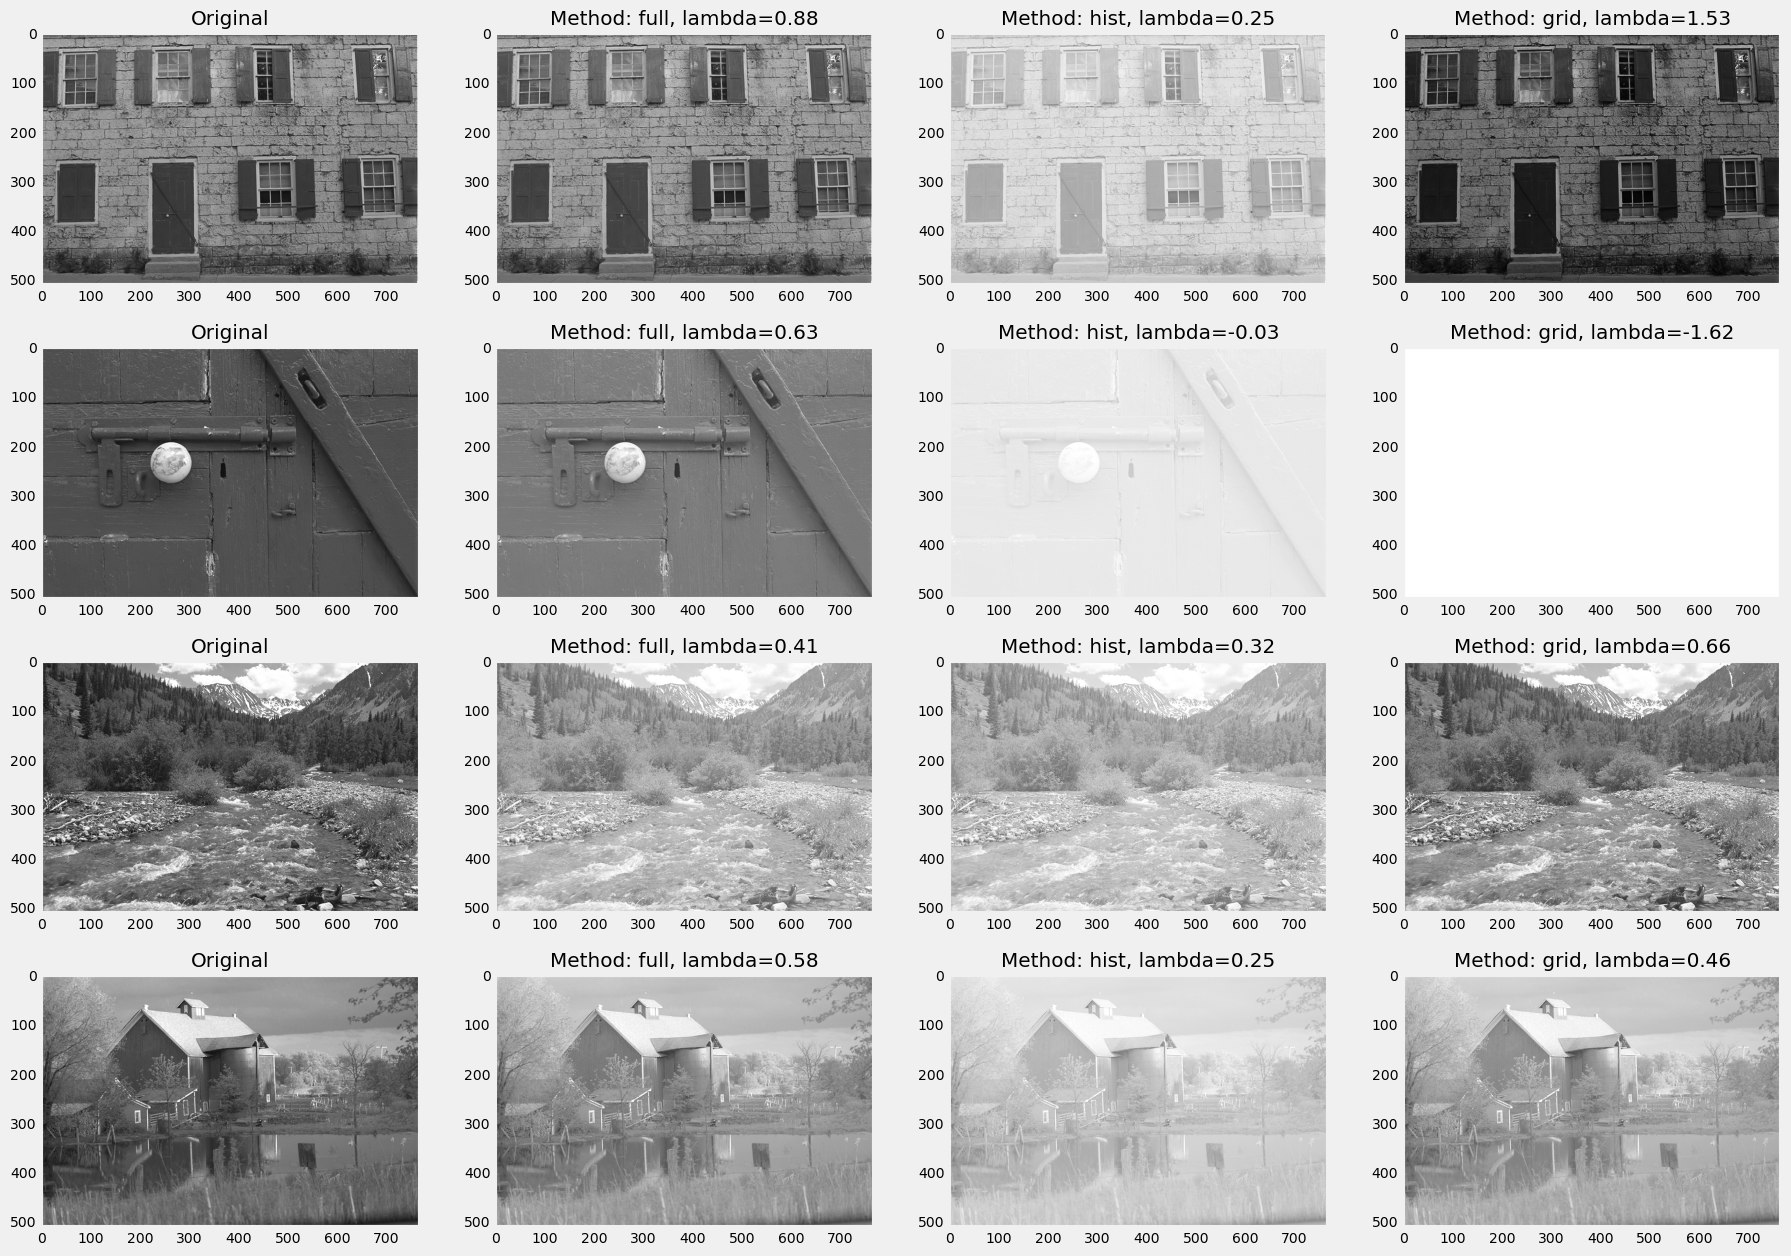
\includegraphics[width=0.7\textwidth]{img_bci_all.png}
        \caption{Transformaciones de la im\'agen 1, 2, 13, y 22. De izquierda a derecha, im\'agen original, m\'etodo de datos completos, m\'etodo de histograma, y m\'etodo de grilla.}
        \label{fig:img_bci_all}
    \end{figure}
\end{frame}

\begin{frame}
    \begin{center}
        {\LARGE\bf ¿Qué valores de $\lambda$ obtenemos?}
    \end{center}
\end{frame}


\begin{frame}{$\lambda$'s obtenidos}
    % \pause
    \begin{figure}[H]
        \centering
        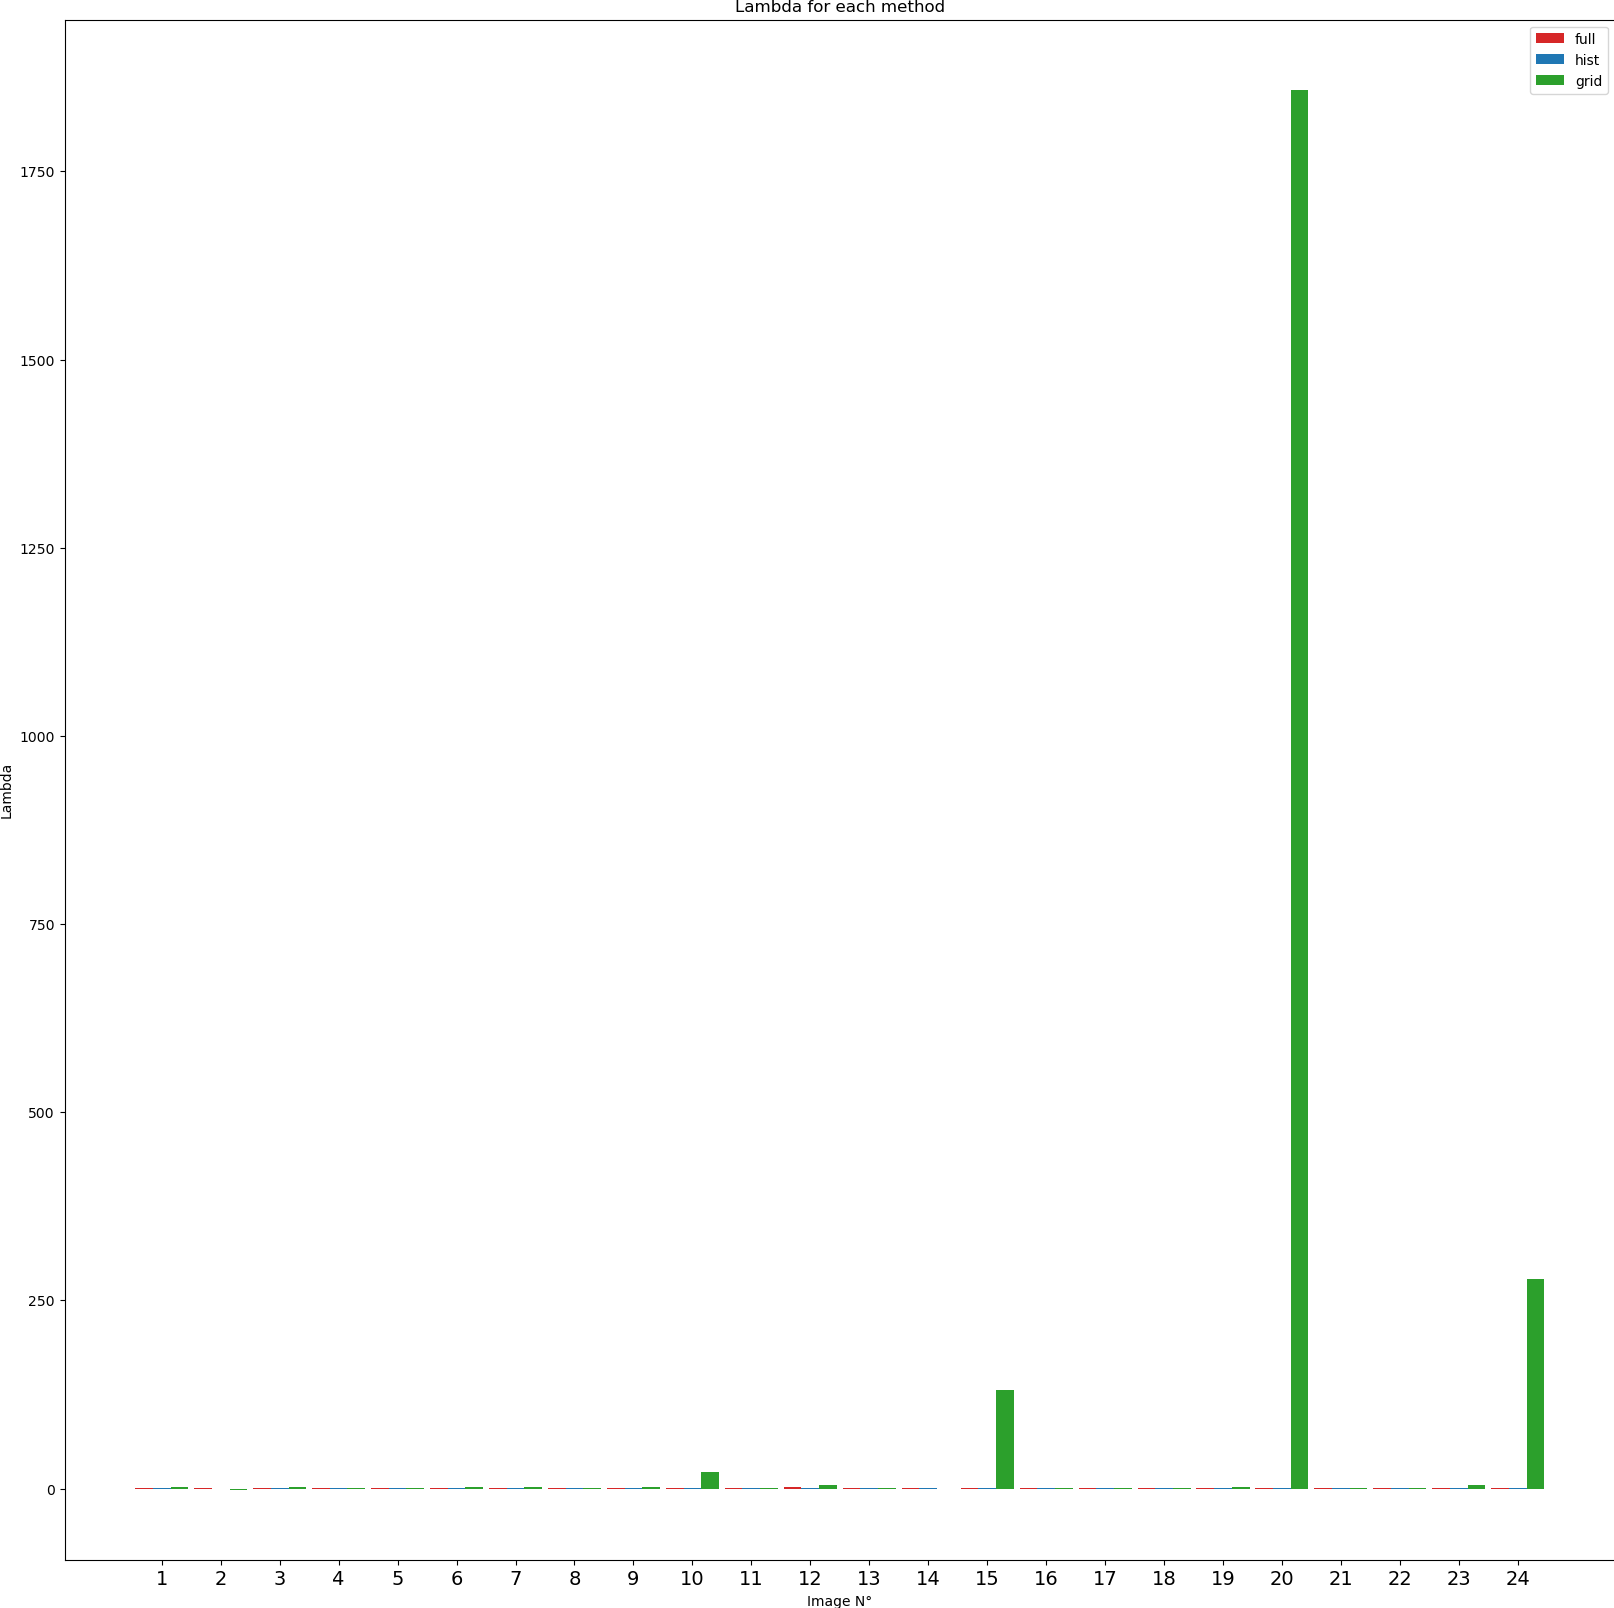
\includegraphics[width=0.6\textwidth]{lambda_noclip.png}
        \caption{Valores de $\lambda$ para todo el banco de im\'agenes. verde es el m\'etodo de grilla, azul es el m\'etodo de histograma, y rojo es el m\'etodo de datos completos.}
        \label{fig:lambda_noclip}
    \end{figure}
    % \pause
    \begin{figure}[H]
        \centering
        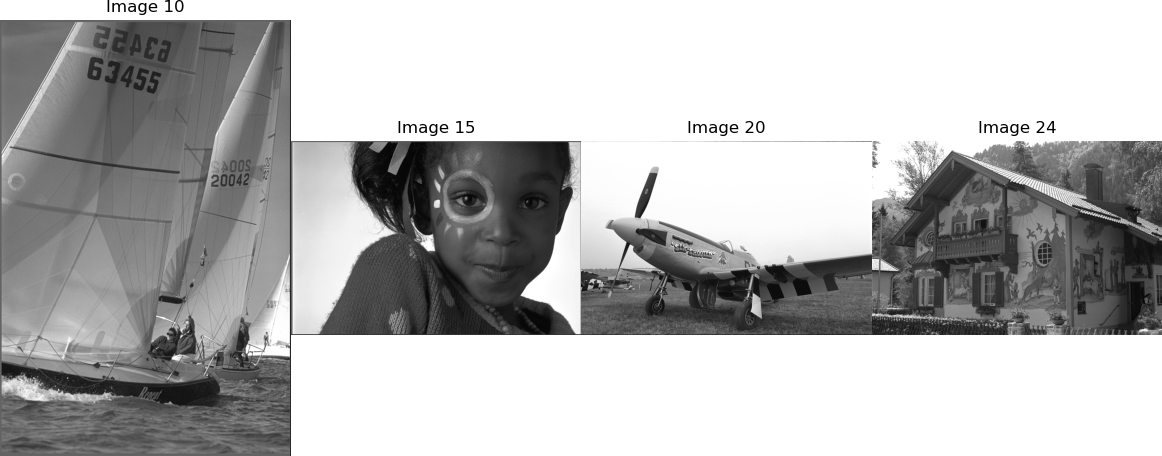
\includegraphics[width=0.9\textwidth]{img_ex_10_15_20_24.png}
        \caption{Transformaciones de las im\'agenes 10, 15, 20, y 24.}
        \label{fig:img_bci_10_15_20}
    \end{figure}

\end{frame}

\begin{frame}{$\lambda$'s obtenidos}
    % \pause
    \begin{figure}[H]
        \centering
        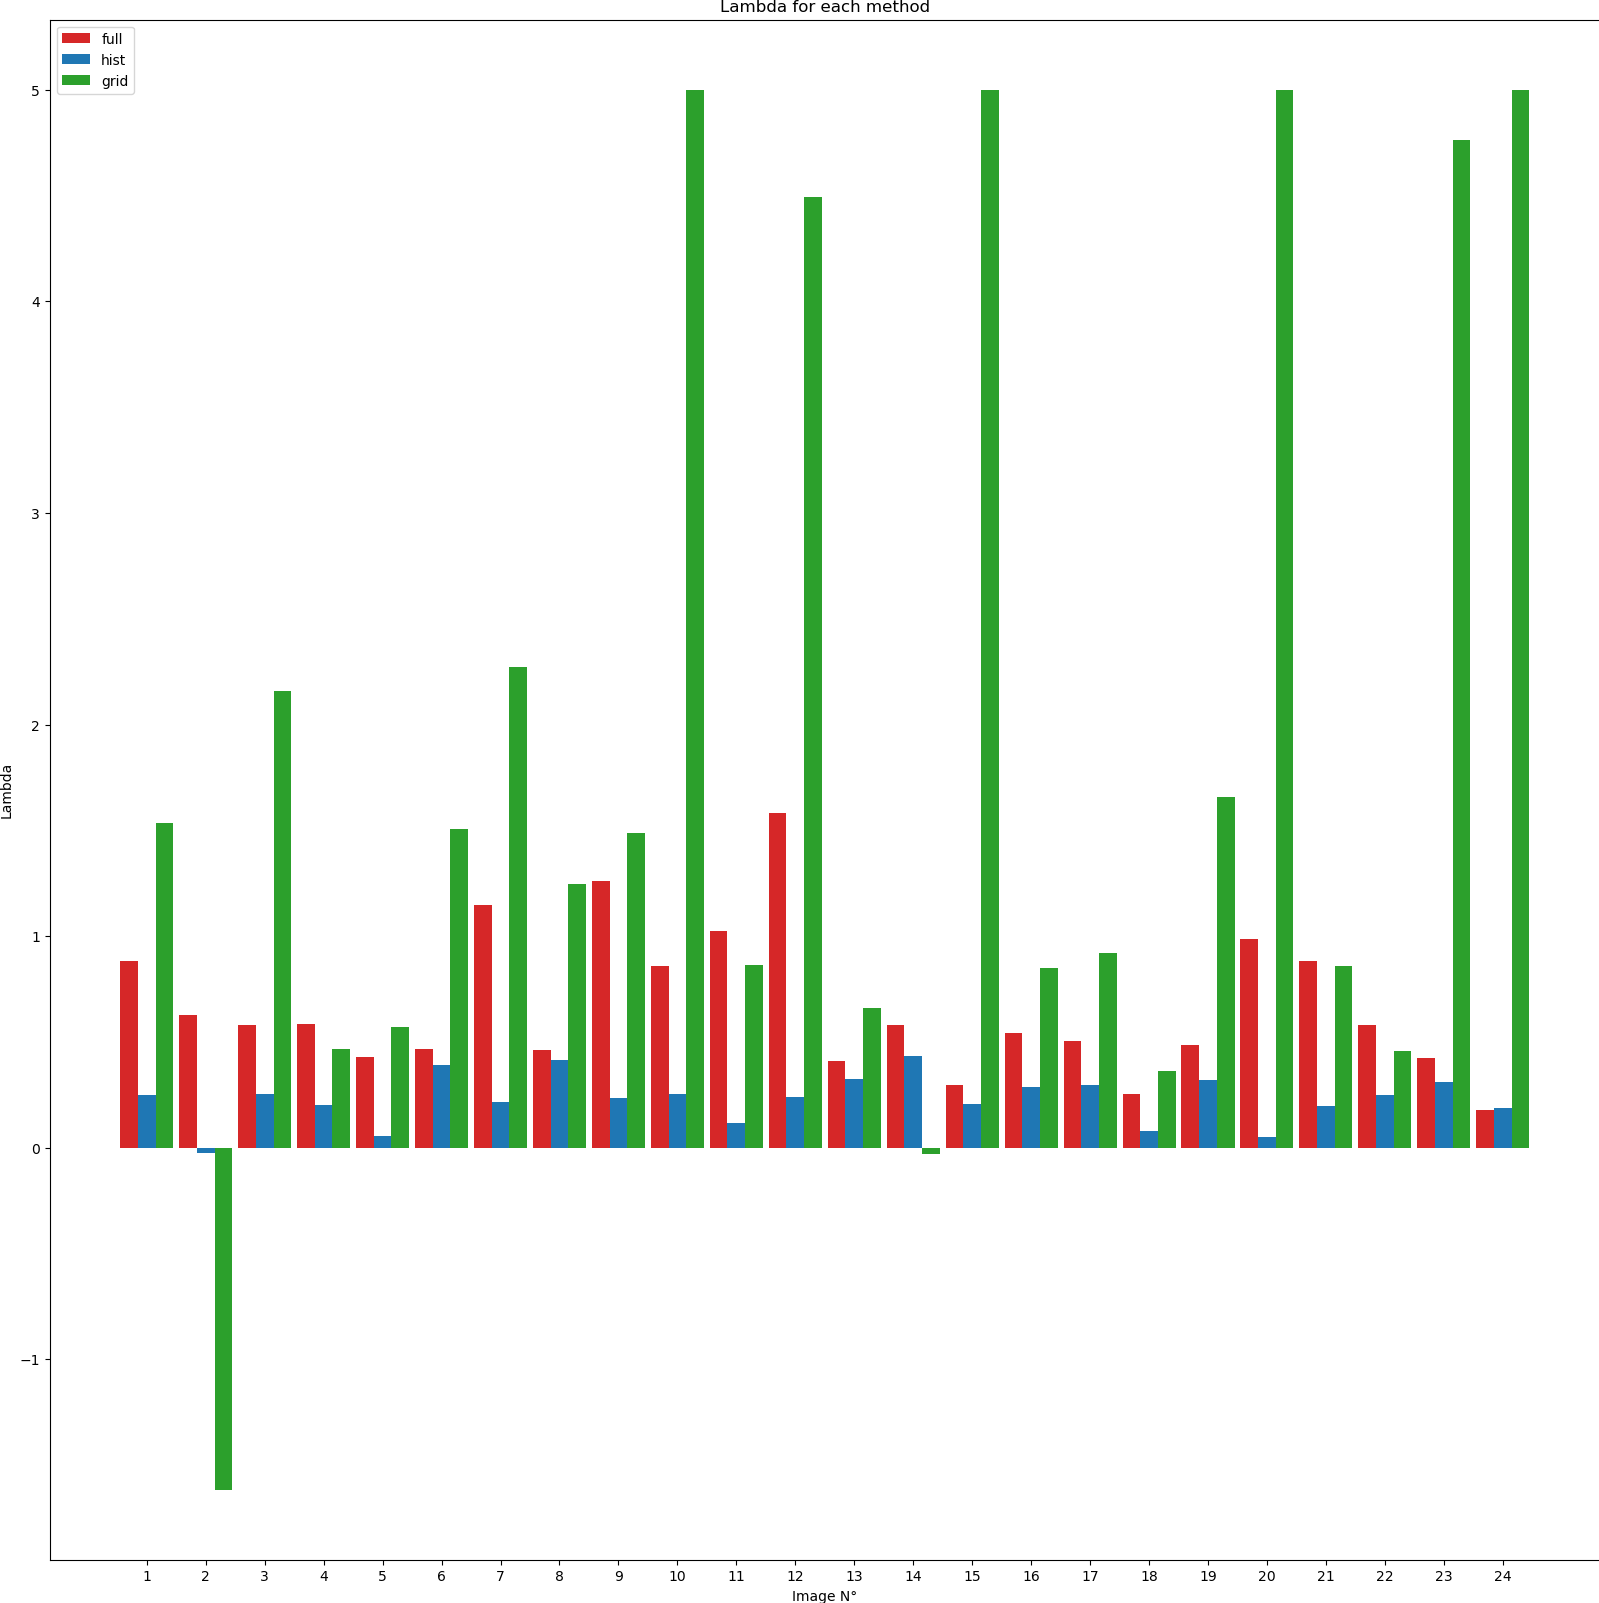
\includegraphics[width=0.5\textwidth]{lambda_clip.png}
        \caption{Valores de $\lambda$ para todo el banco de im\'agenes, cortado en 5. verde es el m\'etodo de grilla, azul es histograma, y rojo es datos completos}
        \label{fig:lambda_clip}
    \end{figure}
\end{frame}


\begin{frame}{Correlaciones}
    \begin{block}{Correlaciones}
        \begin{table}[H]
            \centering
            \begin{tabular}{|l|l|l|l|}
                \hline
                M\'etodo 1 & M\'etodo 2 & Pearson $\rho$ & Valor P \\ \hline
                Completo                  & Histograma                & -0.1305   & 0.5431  \\ 
                Completo                  & Grilla                    & 0.1384    & 0.5191  \\ 
                Histograma                & Grilla                    & -0.3467   & 0.0968  \\ \hline
            \end{tabular}
        \end{table}
    \end{block}
    Notemos que Cheddad et al. (2010), encontró una correlación entre el método completo y el del histograma es de $-0.3022$.
\end{frame}



\section{Experimentos Numéricos}
\begin{frame}
    \begin{center}
        {\LARGE\bf Experimentos Numéricos}
    \end{center}
\end{frame}


\begin{frame}{Experimentos Numéricos}
    % \pause
    Para estos experimentos utilizamos el banco de imágenes mostrado anteriormente. Para cada imagen, hacemos la transformación para un rango de valores, además de los valores de $\lambda$ obtenidos por los métodos de grilla, histograma, y completo.
    % \pause
    \begin{figure}[H]
        \centering
        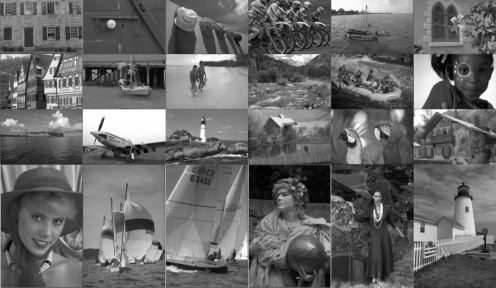
\includegraphics[width=0.4\textwidth]{all_images_grid_bw.png}
    \end{figure}

    Luego,utilizaremos los métodos de correlación de MIC y dCor; comparando el vector completo y el histograma de las imágenes transformadas con la imagen original.
    
    Además se muestra la correlación de Pearson $\rho$ como base de comparación.
\end{frame}

\begin{frame}
    \begin{center}
        {\LARGE\bf Rango de valores para $\lambda$}
    \end{center}
    % \pause
    \begin{center}
        {\Large\bf Comprando los vectores de las imágenes.}
    \end{center}
\end{frame}


\begin{frame}{Experimentos Numéricos}
    % \pause
    
    \begin{figure}[H]
        \centering
        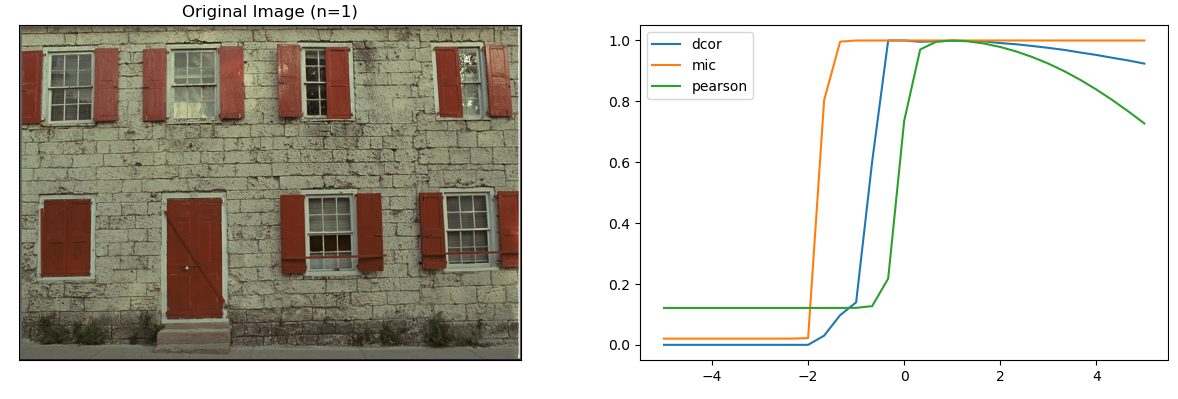
\includegraphics[width=\textwidth]{lam_v_com_one.png}
        \caption{De arriba hacia abajo, imagen 1. A la izquierda la imagen original y a la derecha el valor de $dCor$ (azul), $MIC$ (naranja), y $\rho$ (verde) en el eje y, $\lambda$ en el eje x.}
    \end{figure}
\end{frame}

\begin{frame}{Experimentos Numéricos}
    % \pause
    Comprando los vectores de las imágenes.
    \begin{figure}[H]
        \centering
        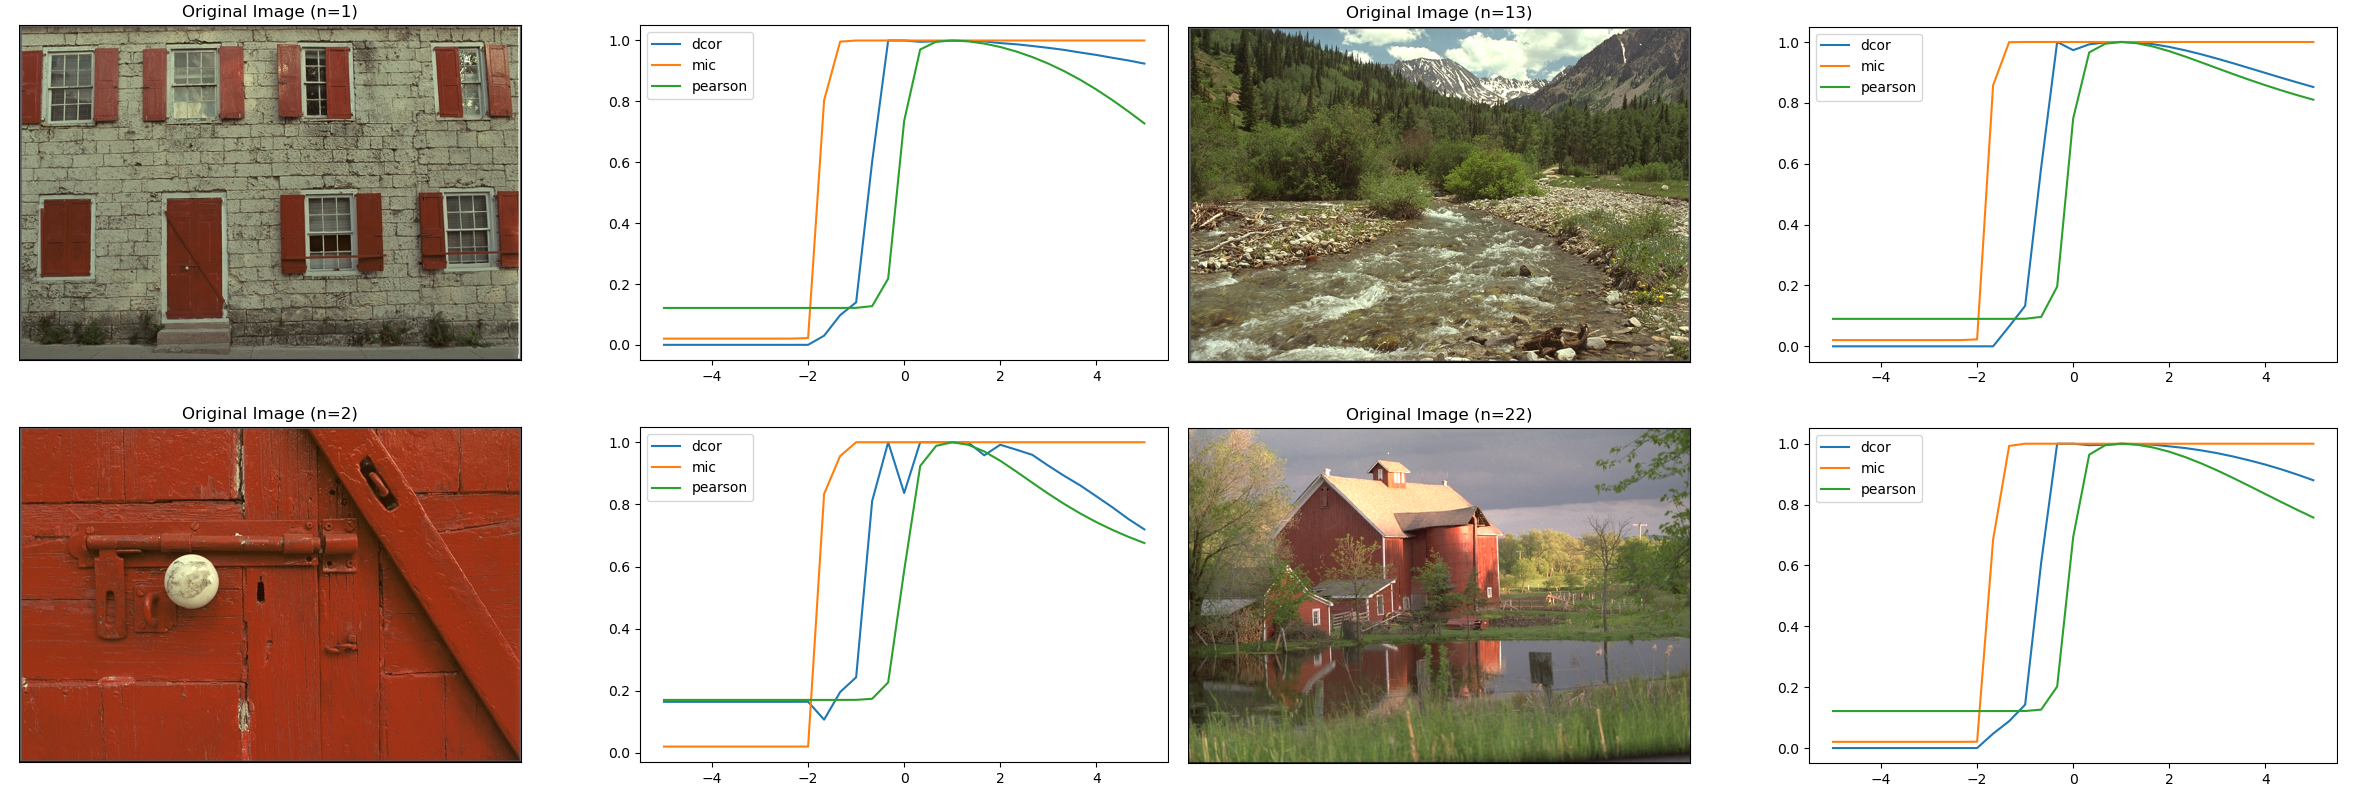
\includegraphics[width=\textwidth]{lam_v_com_all_img.png}
        \caption{De arriba hacia abajo, im\'agenes 1, 2, 13, y 22. A la izquierda la imagen original y a la derecha el valor de $dCor$ (azul), $MIC$ (naranja), y $\rho$ (verde) en el eje y, $\lambda$ en el eje x.}
    \end{figure}
\end{frame}


\begin{frame}
    \begin{center}
        {\LARGE\bf Rango de valores para $\lambda$}
    \end{center}
    % \pause
    \begin{center}
        {\Large\bf Comprando el histograma de las imágenes.}
    \end{center}
\end{frame}
\begin{frame}{Experimentos Numéricos}
    % \pause
    \begin{figure}[H]
        \centering
        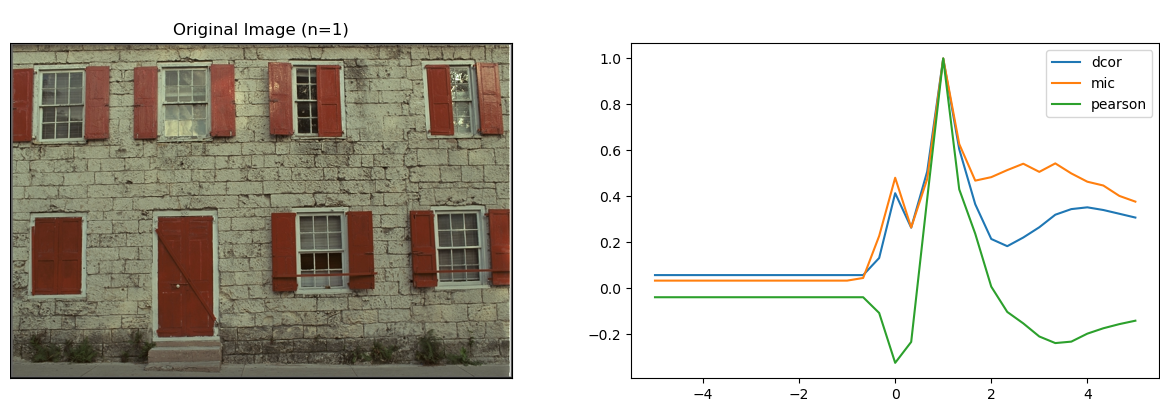
\includegraphics[width=\textwidth]{lam_v_com_one_hist.png}
        \caption{De arriba hacia abajo, im\'agenes 1, 2, 13, y 22. A la izquierda la imagen original y a la derecha el valor de $dCor$ (azul), $MIC$ (naranja), y $\rho$ (verde) en el eje y, $\lambda$ en el eje x.}
    \end{figure}
\end{frame}

\begin{frame}{Experimentos Numéricos}
    % \pause
    \begin{figure}[H]
        \centering
        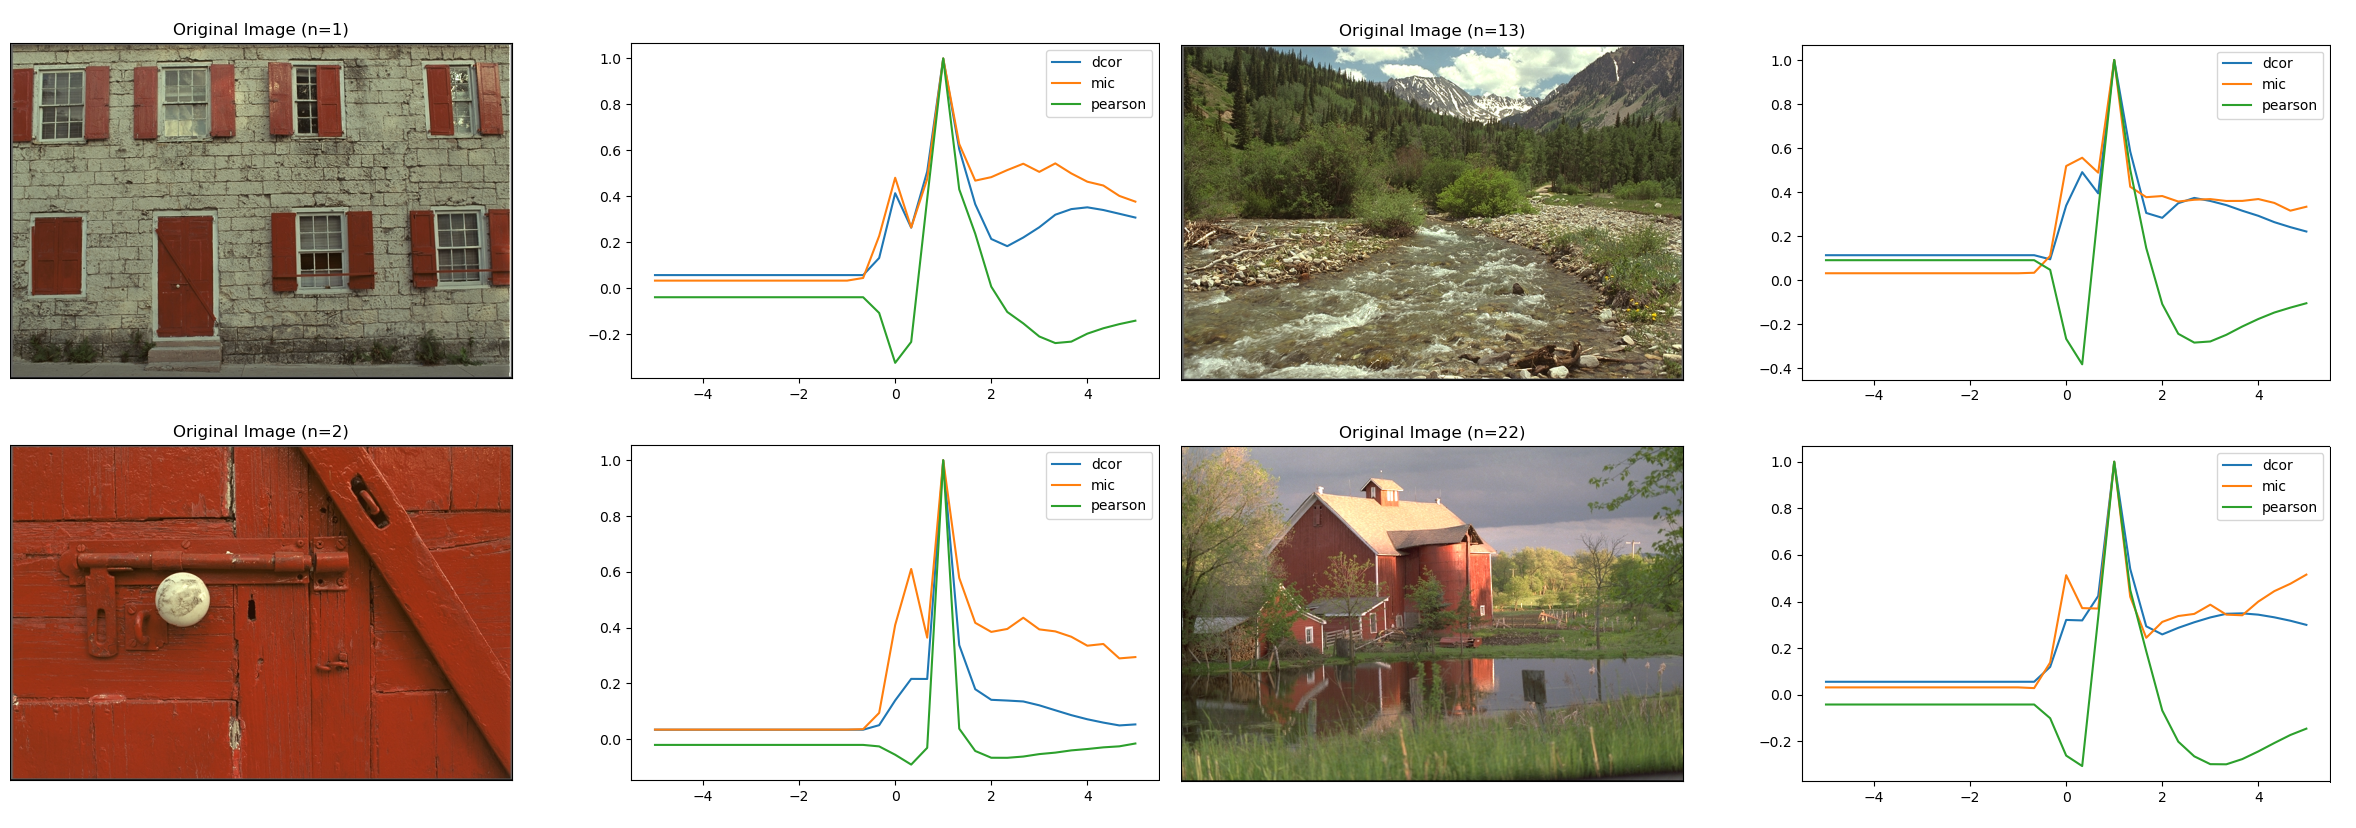
\includegraphics[width=0.8\textwidth]{lam_v_com_all_img_hist.png}
        \caption{De arriba hacia abajo, im\'agenes 1, 2, 13, y 22. A la izquierda la imagen original y a la derecha el valor de $dCor$ (azul), $MIC$ (naranja), y $\rho$ (verde) en el eje y, $\lambda$ en el eje x.}
    \end{figure}
\end{frame}

\begin{frame}
    \begin{center}
        {\LARGE\bf Valores seleccionados de $\lambda$}
    \end{center}
    % \pause
    \begin{center}
        {\Large\bf Comprando los vectores de las imágenes. $\lambda$}
    \end{center}
\end{frame}

\begin{frame}{Experimentos Numéricos}
    % \pause
    \begin{figure}[H]
        \centering
        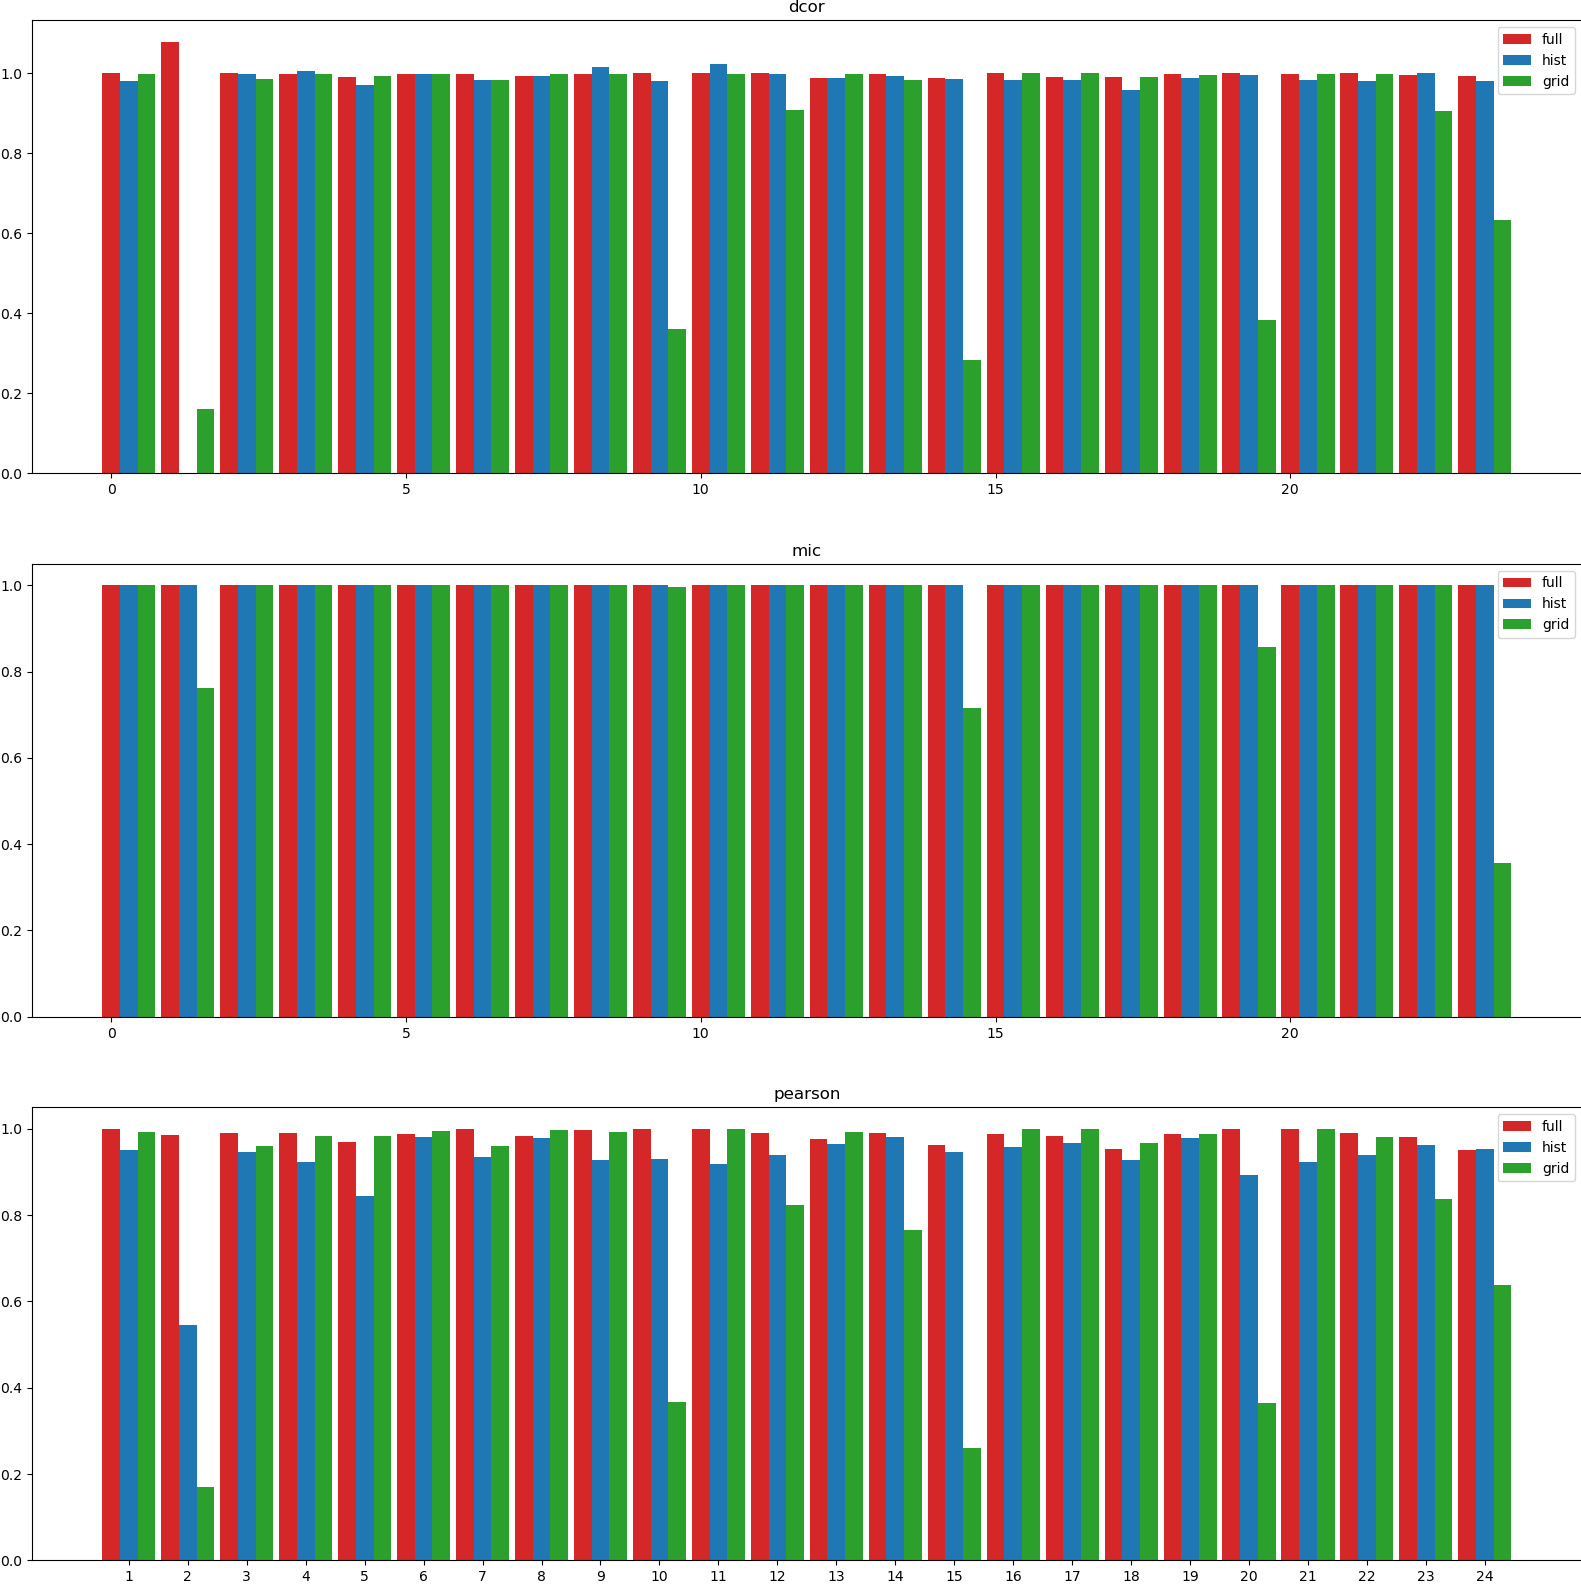
\includegraphics[width=0.6\textwidth]{plot_comparison_full.png}
        \caption{Valores de dcor, mic y pearson para cada imagen usando todo el vector, azul es el metodo para encontrar $\lambda$ con toda la imagen, rojo es el histograma y verde es el grilla.}
    \end{figure}
\end{frame}
\begin{frame}{Experimentos Numéricos}
    Los promedio de los valores de correlación para cada método, comparando los vectores de las imagenes son:
    % \pause
    \begin{block}{Corr.} 
        \begin{table}[H]
            \centering
            \begin{tabular}{|l|l|l|}
                \hline
            Correlaci\'on    & $\lambda$ & Valor  \\    \hline
            dcor    & Completo    & 1.000  \\
            mic     & Completo    & 1.000  \\
            mic     & Histograma  & 1.000  \\
            pearson & Completo    & 0.985 \\
            dcor    & Histograma  & 0.948 \\
            mic     & Grilla      & 0.945  \\
            pearson & Histograma  & 0.925  \\
            dcor    & Grilla      & 0.856  \\
            pearson & Grilla      & 0.945  \\     \hline
    
            \end{tabular}
        \end{table}
    \end{block}
\end{frame}
\begin{frame}
    \begin{center}
        {\LARGE\bf Valores seleccionados de $\lambda$}
    \end{center}
    % \pause
    \begin{center}
        {\Large\bf Comprando el histograms de las imágenes. $\lambda$}
    \end{center}
\end{frame}

\begin{frame}{Experimentos Numéricos}
    % \pause
    \begin{figure}[H]
        \centering
        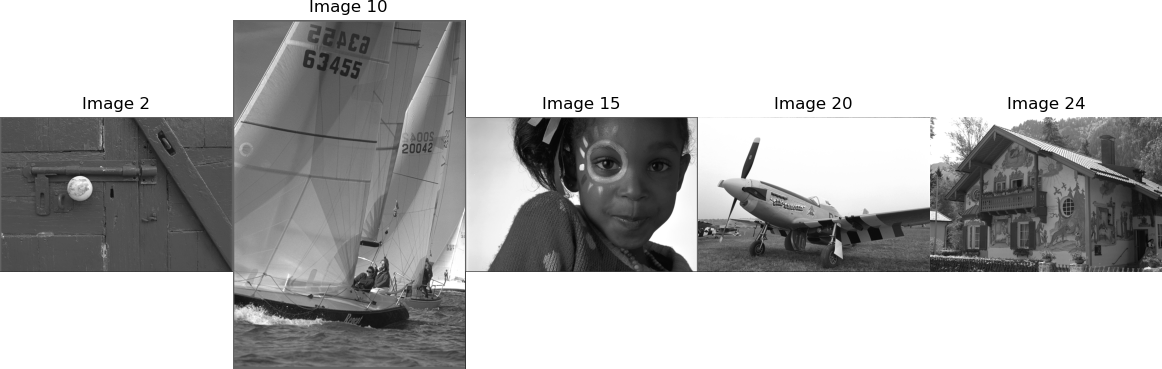
\includegraphics[width=\textwidth]{anomalies_grid.png}
        \caption{De izquierda a derecha, im\'agenes 2, 10, 15, 20, y 24 del banco.}
    \end{figure}
    Estos corresponden a los valores an\'omalos en el m\'etodo de grilla.
\end{frame}


\begin{frame}{Experimentos Numéricos}
    \begin{figure}[H]
        \centering
        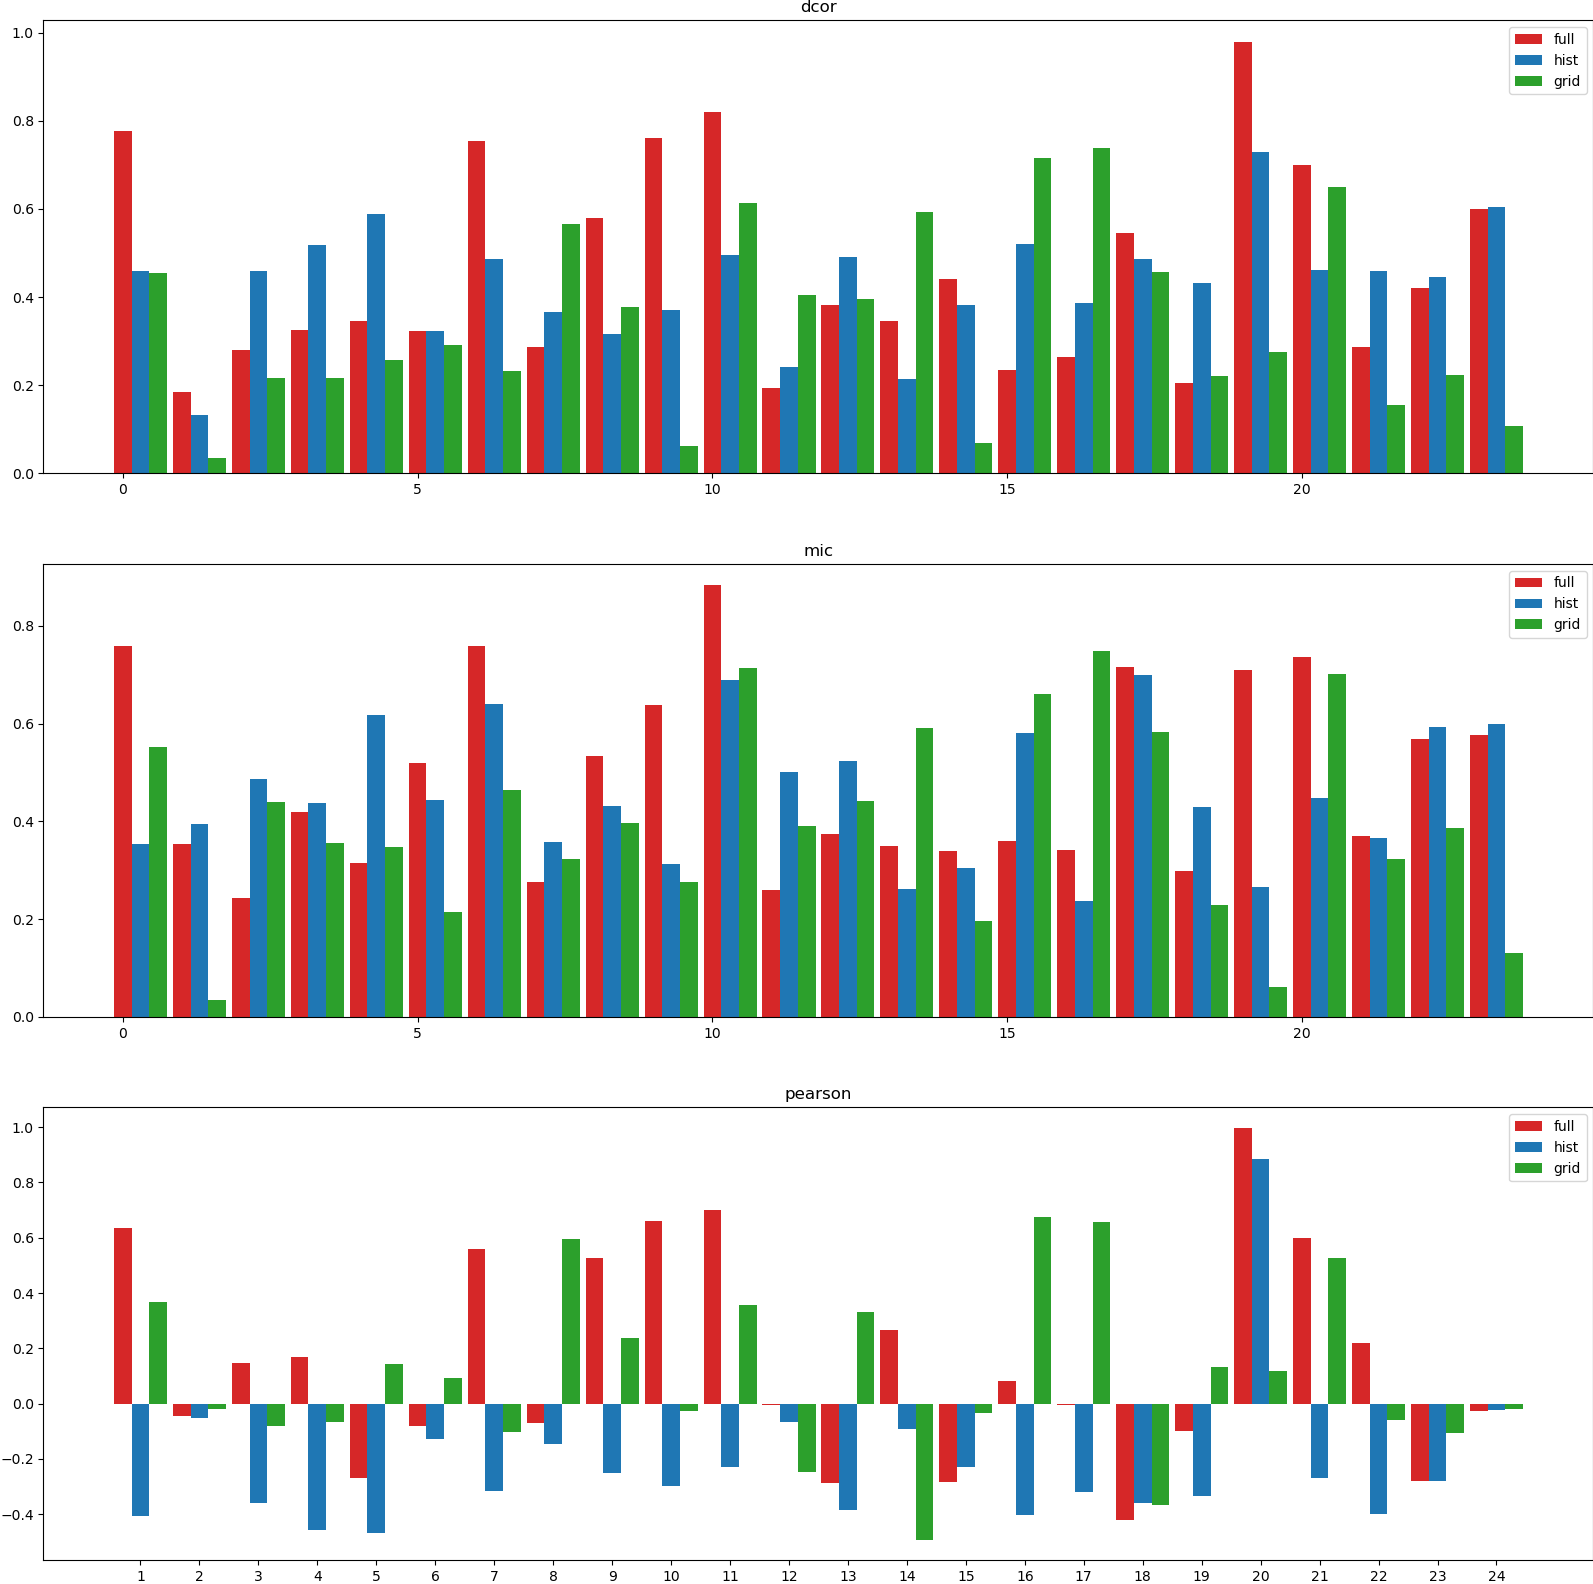
\includegraphics[width=0.6\textwidth]{plot_comparison_hist.png}
        \caption{Valores de dcor, mic y pearson para cada imagen usando el histograma, azul es el metodo para encontrar $\lambda$ con toda la imagen, rojo es el histograma y verde es el grid}
    \end{figure}
\end{frame}

\begin{frame}{Experimentos Numéricos}
    % \pause
    Los promedio de los valores de correlación para cada método, comparando el histograma de las imagenes son:
    % \pause
    \begin{block}{Corr.} 
        \begin{table}[H]
            \centering
            \begin{tabular}{|l|l|l|}\hline
            mic     & Completo    & 0.487  \\\hline
            dcor    & Completo    & 0.459  \\
            mic     & Histograma  & 0.457  \\
            dcor    & Histograma  & 0.431  \\
            mic     & Grilla      & 0.398  \\
            dcor    & Grilla      & 0.346 \\
            pearson & Completo    & 0.108  \\
            pearson & Grilla      & 0.108  \\
            pearson & Histograma  & -0.225 \\\hline
            \end{tabular}
        \end{table}
    \end{block}
\end{frame}

\section{Conlusiones}

\begin{frame}{Conlusiones}
    
    \begin{itemize}
        % \pause
        \item Dentro de un rango para $\lambda$, las transformaciones de Box-Cox están fuertemente corelacionadas con sus primitivas.
        \item Los métodos de selección de $\lambda$ son útiles para encontrar valores que maximizan la correlación entre las imágenes, a excepción del método de grilla, que puede ser \textit{instable}
        % \pause
        \item La transformación de Box-Cox puede ser útil normalizar imágenes, pero hay más trabajo por hacer en este campo.
        % \pause
        \item La comparación entre imágenes es compleja, y no hay un método claro o único para hacerlo.
    \end{itemize}
\end{frame}

\begin{frame}{Trabajos Futuros}
    \begin{itemize}
        % \pause
        \item Explorar otros métodos de selección de $\lambda$. 
        \item Explorar trabajar $\lambda$ como una función $\lambda(x, y)$.
        % \pause
        \item Explorar otros métodos de comparación de imágenes.
        % \pause
    \end{itemize}
    
\end{frame}


\begin{frame}{Bibliografía}
    \begin{thebibliography}{9}
    \bibitem{boxcox}
    Box, G. and Cox, D., 1964. An Analysis of Transformations. Journal of the Royal Statistical Society, 26(2), pp.211-252.
    
    \bibitem{Szekely2009}
    Szekely, G\'abor J and Rizzo, Maria L, 2009. Brownian distance covariance Annals of Applied Statistics, 3(4), pp.1236-1265.

    \bibitem{reshef2011}
    Reshef, D., Reshef, Y., Finucane, H., Grossman, S., McVean, G., Turnbaugh, P., Lander, E., Mitzenmacher, M. and Sabeti, P., 2011. Detecting Novel Associations in Large Data Sets. Science, 334(6062), pp.1518-1524.
    \bibitem[]{cheddad2020}
    Cheddad, A., 2020. On Box-Cox Transformation for Image Normality and Pattern Classification. IEEE Access, 8, pp.154975-154983.
    
    \bibitem[]{juin2009}
    Juin-Der Lee, Hong-Ren Su, Cheng, P., Liou, M., Aston, J., Tsai, A. and Cheng-Yu Chen, 2009. MR Image Segmentation Using a Power Transformation Approach. IEEE Transactions on Medical Imaging, 28(6), pp.894-905.
    \end{thebibliography}
\end{frame}
\end{document}




